% !TeX TXS-program:bibliography = txs:///biber
\documentclass[14pt, russian]{scrartcl}
\let\counterwithout\relax
\let\counterwithin\relax
%\usepackage{lmodern}
\usepackage{float}
\usepackage{xcolor}
\usepackage{extsizes}
\usepackage{subfig}
\usepackage[export]{adjustbox}
\usepackage{tocvsec2} % возможность менять учитываемую глубину разделов в оглавлении
\usepackage[subfigure]{tocloft}
\usepackage[newfloat]{minted}
\removefromtoclist[float]{lol}% must be after loading `minted`.
\captionsetup[listing]{position=top}

\AtBeginEnvironment{figure}{\vspace{0.5cm}}
\AtBeginEnvironment{table}{\vspace{0.5cm}}
\AtBeginEnvironment{listing}{\vspace{0.5cm}}
\AtBeginEnvironment{algorithm}{\vspace{0.5cm}}
\AtBeginEnvironment{minted}{\vspace{-0.5cm}}

\usepackage{fancyvrb}
\usepackage{ulem,bm,mathrsfs,ifsym} %зачеркивания, особо жирный стиль и RSFS начертание
\usepackage{sectsty} % переопределение стилей подразделов
%%%%%%%%%%%%%%%%%%%%%%%

%%% Поля и разметка страницы %%%
\usepackage{pdflscape}                              % Для включения альбомных страниц
\usepackage{geometry}                               % Для последующего задания полей
\geometry{a4paper,tmargin=2cm,bmargin=2cm,lmargin=3cm,rmargin=1cm} % тоже самое, но лучше

%%% Математические пакеты %%%
\usepackage{amsthm,amsfonts,amsmath,amssymb,amscd}  % Математические дополнения от AMS
\usepackage{mathtools}                              % Добавляет окружение multlined
\usepackage[perpage]{footmisc}
%\usepackage{times}

%%%% Установки для размера шрифта 14 pt %%%%
%% Формирование переменных и констант для сравнения (один раз для всех подключаемых файлов)%%
%% должно располагаться до вызова пакета fontspec или polyglossia, потому что они сбивают его работу
%\newlength{\curtextsize}
%\newlength{\bigtextsize}
%\setlength{\bigtextsize}{13pt}
\KOMAoptions{fontsize=14pt}

\makeatletter
\def\showfontsize{\f@size{} point}
\makeatother

\makeatletter
\setlength{\@fptop}{0pt}
\makeatother

%\makeatletter
%\show\f@size                                       % неплохо для отслеживания, но вызывает стопорение процесса, если документ компилируется без команды  -interaction=nonstopmode 
%\setlength{\curtextsize}{\f@size pt}
%\makeatother

%шрифт times
\usepackage{tempora}
%\usepackage{pscyr}
%\setmainfont[Ligatures={TeX,Historic}]{Times New Roman}

   %%% Решение проблемы копирования текста в буфер кракозябрами
%    \input glyphtounicode.tex
%    \input glyphtounicode-cmr.tex %from pdfx package
%    \pdfgentounicode=1
    \usepackage{cmap}                               % Улучшенный поиск русских слов в полученном pdf-файле
    \usepackage[T1]{fontenc}                       % Поддержка русских букв
    \usepackage[utf8]{inputenc}                     % Кодировка utf8
    \usepackage[english, main=russian]{babel}            % Языки: русский, английский
%   \IfFileExists{pscyr.sty}{\usepackage{pscyr}}{}  % Красивые русские шрифты
%\renewcommand{\rmdefault}{ftm}
%%% Оформление абзацев %%%
\usepackage{indentfirst}                            % Красная строка
%\usepackage{eskdpz}

%%% Таблицы %%%
\usepackage{longtable}                              % Длинные таблицы
\usepackage{multirow,makecell,array}                % Улучшенное форматирование таблиц
\usepackage{booktabs}                               % Возможность оформления таблиц в классическом книжном стиле (при правильном использовании не противоречит ГОСТ)

%%% Общее форматирование
\usepackage{soulutf8}                               % Поддержка переносоустойчивых подчёркиваний и зачёркиваний
\usepackage{icomma}                                 % Запятая в десятичных дробях



%%% Изображения %%%
\usepackage{graphicx}                               % Подключаем пакет работы с графикой
\usepackage{wrapfig}

%%% Списки %%%
\usepackage{enumitem}

%%% Подписи %%%
\usepackage{caption}                                % Для управления подписями (рисунков и таблиц) % Может управлять номерами рисунков и таблиц с caption %Иногда может управлять заголовками в списках рисунков и таблиц
%% Использование:
%\begin{table}[h!]\ContinuedFloat - чтобы не переключать счетчик
%\captionsetup{labelformat=continued}% должен стоять до самого caption
%\caption{}
% либо ручками \caption*{Продолжение таблицы~\ref{...}.} :)

%%% Интервалы %%%
\addto\captionsrussian{%
  \renewcommand{\listingname}{Листинг}%
}
%%% Счётчики %%%
\usepackage[figure,table,section]{totalcount}               % Счётчик рисунков и таблиц
\DeclareTotalCounter{lstlisting}
\usepackage{totcount}                               % Пакет создания счётчиков на основе последнего номера подсчитываемого элемента (может требовать дважды компилировать документ)
\usepackage{totpages}                               % Счётчик страниц, совместимый с hyperref (ссылается на номер последней страницы). Желательно ставить последним пакетом в преамбуле

%%% Продвинутое управление групповыми ссылками (пока только формулами) %%%
%% Кодировки и шрифты %%%

%   \newfontfamily{\cyrillicfont}{Times New Roman}
%   \newfontfamily{\cyrillicfonttt}{CMU Typewriter Text}
	%\setmainfont{Times New Roman}
	%\newfontfamily\cyrillicfont{Times New Roman}
	%\setsansfont{Times New Roman}                    %% задаёт шрифт без засечек
%	\setmonofont{Liberation Mono}               %% задаёт моноширинный шрифт
%    \IfFileExists{pscyr.sty}{\renewcommand{\rmdefault}{ftm}}{}
%%% Интервалы %%%
%linespread-реализация ближе к реализации полуторного интервала в ворде.
%setspace реализация заточена под шрифты 10, 11, 12pt, под остальные кегли хуже, но всё же ближе к типографской классике. 
\linespread{1.3}                    % Полуторный интервал (ГОСТ Р 7.0.11-2011, 5.3.6)
%\renewcommand{\@biblabel}[1]{#1}

%%% Гиперссылки %%%
\usepackage{hyperref}

%%% Выравнивание и переносы %%%
\sloppy                             % Избавляемся от переполнений
\clubpenalty=10000                  % Запрещаем разрыв страницы после первой строки абзаца
\widowpenalty=10000                 % Запрещаем разрыв страницы после последней строки абзаца

\makeatletter % малые заглавные, small caps shape
\let\@@scshape=\scshape
\renewcommand{\scshape}{%
  \ifnum\strcmp{\f@series}{bx}=\z@
    \usefont{T1}{cmr}{bx}{sc}%
  \else
    \ifnum\strcmp{\f@shape}{it}=\z@
      \fontshape{scsl}\selectfont
    \else
      \@@scshape
    \fi
  \fi}
\makeatother

%%% Подписи %%%
%\captionsetup{%
%singlelinecheck=off,                % Многострочные подписи, например у таблиц
%skip=2pt,                           % Вертикальная отбивка между подписью и содержимым рисунка или таблицы определяется ключом
%justification=centering,            % Центрирование подписей, заданных командой \caption
%}
%%%        Подключение пакетов                 %%%
\usepackage{ifthen}                 % добавляет ifthenelse
%%% Инициализирование переменных, не трогать!  %%%
\newcounter{intvl}
\newcounter{otstup}
\newcounter{contnumeq}
\newcounter{contnumfig}
\newcounter{contnumtab}
\newcounter{pgnum}
\newcounter{bibliosel}
\newcounter{chapstyle}
\newcounter{headingdelim}
\newcounter{headingalign}
\newcounter{headingsize}
\newcounter{tabcap}
\newcounter{tablaba}
\newcounter{tabtita}
%%%%%%%%%%%%%%%%%%%%%%%%%%%%%%%%%%%%%%%%%%%%%%%%%%

%%% Область упрощённого управления оформлением %%%

%% Интервал между заголовками и между заголовком и текстом
% Заголовки отделяют от текста сверху и снизу тремя интервалами (ГОСТ Р 7.0.11-2011, 5.3.5)
\setcounter{intvl}{3}               % Коэффициент кратности к размеру шрифта

%% Отступы у заголовков в тексте
\setcounter{otstup}{0}              % 0 --- без отступа; 1 --- абзацный отступ

%% Нумерация формул, таблиц и рисунков
\setcounter{contnumeq}{1}           % Нумерация формул: 0 --- пораздельно (во введении подряд, без номера раздела); 1 --- сквозная нумерация по всей диссертации
\setcounter{contnumfig}{1}          % Нумерация рисунков: 0 --- пораздельно (во введении подряд, без номера раздела); 1 --- сквозная нумерация по всей диссертации
\setcounter{contnumtab}{1}          % Нумерация таблиц: 0 --- пораздельно (во введении подряд, без номера раздела); 1 --- сквозная нумерация по всей диссертации

%% Оглавление
\setcounter{pgnum}{0}               % 0 --- номера страниц никак не обозначены; 1 --- Стр. над номерами страниц (дважды компилировать после изменения)

%% Библиография
\setcounter{bibliosel}{1}           % 0 --- встроенная реализация с загрузкой файла через движок bibtex8; 1 --- реализация пакетом biblatex через движок biber

%% Текст и форматирование заголовков
\setcounter{chapstyle}{1}           % 0 --- разделы только под номером; 1 --- разделы с названием "Глава" перед номером
\setcounter{headingdelim}{1}        % 0 --- номер отделен пропуском в 1em или \quad; 1 --- номера разделов и приложений отделены точкой с пробелом, подразделы пропуском без точки; 2 --- номера разделов, подразделов и приложений отделены точкой с пробелом.

%% Выравнивание заголовков в тексте
\setcounter{headingalign}{0}        % 0 --- по центру; 1 --- по левому краю

%% Размеры заголовков в тексте
\setcounter{headingsize}{0}         % 0 --- по ГОСТ, все всегда 14 пт; 1 --- пропорционально изменяющийся размер в зависимости от базового шрифта

%% Подпись таблиц
\setcounter{tabcap}{0}              % 0 --- по ГОСТ, номер таблицы и название разделены тире, выровнены по левому краю, при необходимости на нескольких строках; 1 --- подпись таблицы не по ГОСТ, на двух и более строках, дальнейшие настройки: 
%Выравнивание первой строки, с подписью и номером
\setcounter{tablaba}{2}             % 0 --- по левому краю; 1 --- по центру; 2 --- по правому краю
%Выравнивание строк с самим названием таблицы
\setcounter{tabtita}{1}             % 0 --- по левому краю; 1 --- по центру; 2 --- по правому краю

%%% Рисунки %%%
\DeclareCaptionLabelSeparator*{emdash}{~--- }             % (ГОСТ 2.105, 4.3.1)
\captionsetup[figure]{labelsep=emdash,font=onehalfspacing,position=bottom}

%%% Таблицы %%%
\ifthenelse{\equal{\thetabcap}{0}}{%
    \newcommand{\tabcapalign}{\raggedright}  % по левому краю страницы или аналога parbox
}

\ifthenelse{\equal{\thetablaba}{0} \AND \equal{\thetabcap}{1}}{%
    \newcommand{\tabcapalign}{\raggedright}  % по левому краю страницы или аналога parbox
}

\ifthenelse{\equal{\thetablaba}{1} \AND \equal{\thetabcap}{1}}{%
    \newcommand{\tabcapalign}{\centering}    % по центру страницы или аналога parbox
}

\ifthenelse{\equal{\thetablaba}{2} \AND \equal{\thetabcap}{1}}{%
    \newcommand{\tabcapalign}{\raggedleft}   % по правому краю страницы или аналога parbox
}

\ifthenelse{\equal{\thetabtita}{0} \AND \equal{\thetabcap}{1}}{%
    \newcommand{\tabtitalign}{\raggedright}  % по левому краю страницы или аналога parbox
}

\ifthenelse{\equal{\thetabtita}{1} \AND \equal{\thetabcap}{1}}{%
    \newcommand{\tabtitalign}{\centering}    % по центру страницы или аналога parbox
}

\ifthenelse{\equal{\thetabtita}{2} \AND \equal{\thetabcap}{1}}{%
    \newcommand{\tabtitalign}{\raggedleft}   % по правому краю страницы или аналога parbox
}

\DeclareCaptionFormat{tablenocaption}{\tabcapalign #1\strut}        % Наименование таблицы отсутствует
\ifthenelse{\equal{\thetabcap}{0}}{%
    \DeclareCaptionFormat{tablecaption}{\tabcapalign #1#2#3}
    \captionsetup[table]{labelsep=emdash}                       % тире как разделитель идентификатора с номером от наименования
}{%
    \DeclareCaptionFormat{tablecaption}{\tabcapalign #1#2\par%  % Идентификатор таблицы на отдельной строке
        \tabtitalign{#3}}                                       % Наименование таблицы строкой ниже
    \captionsetup[table]{labelsep=space}                        % пробельный разделитель идентификатора с номером от наименования
}
\captionsetup[table]{format=tablecaption,singlelinecheck=off,font=onehalfspacing,position=top,skip=-5pt}  % многострочные наименования и прочее
\DeclareCaptionLabelFormat{continued}{Продолжение таблицы~#2}
\setlength{\belowcaptionskip}{.2cm}
\setlength{\intextsep}{0ex}

%%% Подписи подрисунков %%%
\renewcommand{\thesubfigure}{\asbuk{subfigure}}           % Буквенные номера подрисунков
\captionsetup[subfigure]{font={normalsize},               % Шрифт подписи названий подрисунков (не отличается от основного)
    labelformat=brace,                                    % Формат обозначения подрисунка
    justification=centering,                              % Выключка подписей (форматирование), один из вариантов            
}
%\DeclareCaptionFont{font12pt}{\fontsize{12pt}{13pt}\selectfont} % объявляем шрифт 12pt для использования в подписях, тут же надо интерлиньяж объявлять, если не наследуется
%\captionsetup[subfigure]{font={font12pt}}                 % Шрифт подписи названий подрисунков (всегда 12pt)

%%% Настройки гиперссылок %%%

\definecolor{linkcolor}{rgb}{0.0,0,0}
\definecolor{citecolor}{rgb}{0,0.0,0}
\definecolor{urlcolor}{rgb}{0,0,0}

\hypersetup{
    linktocpage=true,           % ссылки с номера страницы в оглавлении, списке таблиц и списке рисунков
%    linktoc=all,                % both the section and page part are links
%    pdfpagelabels=false,        % set PDF page labels (true|false)
    plainpages=true,           % Forces page anchors to be named by the Arabic form  of the page number, rather than the formatted form
    colorlinks,                 % ссылки отображаются раскрашенным текстом, а не раскрашенным прямоугольником, вокруг текста
    linkcolor={linkcolor},      % цвет ссылок типа ref, eqref и подобных
    citecolor={citecolor},      % цвет ссылок-цитат
    urlcolor={urlcolor},        % цвет гиперссылок
    pdflang={ru},
}
\urlstyle{same}
%%% Шаблон %%%
%\DeclareRobustCommand{\todo}{\textcolor{red}}       % решаем проблему превращения названия цвета в результате \MakeUppercase, http://tex.stackexchange.com/a/187930/79756 , \DeclareRobustCommand protects \todo from expanding inside \MakeUppercase
\setlength{\parindent}{2.5em}                       % Абзацный отступ. Должен быть одинаковым по всему тексту и равен пяти знакам (ГОСТ Р 7.0.11-2011, 5.3.7).

%%% Списки %%%
% Используем дефис для ненумерованных списков (ГОСТ 2.105-95, 4.1.7)
%\renewcommand{\labelitemi}{\normalfont\bfseries~{---}} 
\renewcommand{\labelitemi}{\bfseries~{---}} 
\setlist{nosep,%                                    % Единый стиль для всех списков (пакет enumitem), без дополнительных интервалов.
    labelindent=\parindent,leftmargin=*%            % Каждый пункт, подпункт и перечисление записывают с абзацного отступа (ГОСТ 2.105-95, 4.1.8)
}
%%%%%%%%%%%%%%%%%%%%%%
%\usepackage{xltxtra} % load xunicode

\usepackage{ragged2e}
\usepackage[explicit]{titlesec}
\usepackage{placeins}
\usepackage{url}
\usepackage{xparse}
\usepackage{csquotes}

\usepackage{listingsutf8}
\usepackage{url} %пакеты расширений
\usepackage{algorithm, algorithmicx}
\usepackage[noend]{algpseudocode}
\usepackage{blkarray}
\usepackage{chngcntr}
\usepackage{tabularx}
\usepackage[backend=biber, 
    bibstyle=gost-numeric,
    citestyle=nature]{biblatex}
\newcommand*\template[1]{\text{<}#1\text{>}}
  
\titleformat{name=\section,numberless}[block]{\normalfont\Large\centering}{}{0em}{#1}
\titleformat{\section}[block]{\normalfont\Large\bfseries\raggedright}{}{0em}{\thesection\hspace{0.25em}#1}
\titleformat{\subsection}[block]{\normalfont\Large\bfseries\raggedright}{}{0em}{\thesubsection\hspace{0.25em}#1}
\titleformat{\subsubsection}[block]{\normalfont\large\bfseries\raggedright}{}{0em}{\thesubsubsection\hspace{0.25em}#1}

\let\Algorithm\algorithm
\renewcommand\algorithm[1][]{\Algorithm[#1]\setstretch{1.5}}
%\renewcommand{\listingscaption}{Листинг}

\usepackage{pifont}
\usepackage{calc}
\usepackage{suffix}
\usepackage{csquotes}
\DeclareQuoteStyle{russian}
    {\guillemotleft}{\guillemotright}[0.025em]
    {\quotedblbase}{\textquotedblleft}
\ExecuteQuoteOptions{style=russian}
\newcommand{\enq}[1]{\enquote{#1}}  
\newcommand{\eng}[1]{\begin{english}#1\end{english}}
% Подчиненные счетчики в окружениях http://old.kpfu.ru/journals/izv_vuz/arch/sample1251.tex
\newcounter{cTheorem} 
\newcounter{cDefinition}
\newcounter{cConsequent}
\newcounter{cExample}
\newcounter{cLemma}
\newcounter{cConjecture}
\newtheorem{Theorem}{Теорема}[cTheorem]
\newtheorem{Definition}{Определение}[cDefinition]
\newtheorem{Consequent}{Следствие}[cConsequent]
\newtheorem{Example}{Пример}[cExample]
\newtheorem{Lemma}{Лемма}[cLemma]
\newtheorem{Conjecture}{Гипотеза}[cConjecture]

\renewcommand{\theTheorem}{\arabic{Theorem}}
\renewcommand{\theDefinition}{\arabic{Definition}}
\renewcommand{\theConsequent}{\arabic{Consequent}}
\renewcommand{\theExample}{\arabic{Example}}
\renewcommand{\theLemma}{\arabic{Lemma}}
\renewcommand{\theConjecture}{\arabic{Conjecture}}
%\makeatletter
\NewDocumentCommand{\Newline}{}{\text{\\}}
\newcommand{\sequence}[2]{\ensuremath \left(#1,\ \dots,\ #2\right)}

\definecolor{mygreen}{rgb}{0,0.6,0}
\definecolor{mygray}{rgb}{0.5,0.5,0.5}
\definecolor{mymauve}{rgb}{0.58,0,0.82}
\renewcommand{\listalgorithmname}{Список алгоритмов}
\floatname{algorithm}{Листинг}
\renewcommand{\lstlistingname}{Листинг}
\renewcommand{\thealgorithm}{\arabic{algorithm}}

\newcommand{\refAlgo}[1]{(листинг \ref{#1})}
\newcommand{\refImage}[1]{(рисунок \ref{#1})}

\renewcommand{\theenumi}{\arabic{enumi}.}% Меняем везде перечисления на цифра.цифра	
\renewcommand{\labelenumi}{\arabic{enumi}.}% Меняем везде перечисления на цифра.цифра
\renewcommand{\theenumii}{\arabic{enumii}}% Меняем везде перечисления на цифра.цифра
\renewcommand{\labelenumii}{(\arabic{enumii})}% Меняем везде перечисления на цифра.цифра
\renewcommand{\theenumiii}{\roman{enumiii}}% Меняем везде перечисления на цифра.цифра
\renewcommand{\labelenumiii}{(\roman{enumiii})}% Меняем везде перечисления на цифра.цифра
%\newfontfamily\AnkaCoder[Path=src/fonts/]{AnkaCoder-r.ttf}
\renewcommand{\labelitemi}{---}
\renewcommand{\labelitemii}{---}

%\usepackage{courier}

\lstdefinelanguage{Refal}{
  alsodigit = {.,<,>},
  morekeywords = [1]{ENTRY},
  morekeywords = [2]{Go, Put, Get, Open, Close, Arg, Add, Sub, Mul, Div, Symb, Explode, Implode},
  %keyword4
  morekeywords = [3]{<,>},
  %keyword5
  morekeywords = [4]{e.,t.,s.},
  sensitive = true,
  morecomment = [l]{*},
  morecomment = [s]{/*}{*/},
  commentstyle = \color{mygreen},
  morestring = [b]",
  morestring = [b]',
  stringstyle = \color{purple}
}

\makeatletter
\def\p@subsection{}
\def\p@subsubsection{\thesection\,\thesubsection\,}
\makeatother
\newcommand{\prog}[1]{{\ttfamily\small#1}}
\lstset{ %
  backgroundcolor=\color{white},   % choose the background color; you must add \usepackage{color} or \usepackage{xcolor}
  basicstyle=\ttfamily\footnotesize, 
  %basicstyle=\footnotesize\AnkaCoder,        % the size of the fonts that are used for the code
  breakatwhitespace=false,         % sets if automatic breaks shoulbd only happen at whitespace
  breaklines=true,                 % sets automatic line breaking
  captionpos=top,                    % sets the caption-position to bottom
  commentstyle=\color{mygreen},    % comment style
  deletekeywords={...},            % if you want to delete keywords from the given language
  escapeinside={\%*}{*)},          % if you want to add LaTeX within your code
  extendedchars=true,              % lets you use non-ASCII characters; for 8-bits encodings only, does not work with UTF-8
  inputencoding=utf8,
  frame=single,                    % adds a frame around the code
  keepspaces=true,                 % keeps spaces in text, useful for keeping indentation of code (possibly needs columns=flexible)
  keywordstyle=\bf,       % keyword style
  language=Refal,                    % the language of the code
  morekeywords={<,>,ENTRY,Go,Arg, Open, Close, e., s., t., Get, Put}, 
  							       % if you want to add more keywords to the set
  numbers=left,                    % where to put the line-numbers; possible values are (none, left, right)
  numbersep=5pt,                   % how far the line-numbers are from the code
  xleftmargin=25pt,
  xrightmargin=25pt,
  numberstyle=\small\color{black}, % the style that is used for the line-numbers
  rulecolor=\color{black},         % if not set, the frame-color may be changed on line-breaks within not-black text (e.g. comments (green here))
  showspaces=false,                % show spaces everywhere adding particular underscores; it overrides 'showstringspaces'
  showstringspaces=false,          % underline spaces within strings only
  showtabs=false,                  % show tabs within strings adding particular underscores
  stepnumber=1,                    % the step between two line-numbers. If it's 1, each line will be numbered
  stringstyle=\color{mymauve},     % string literal style
  tabsize=8,                       % sets default tabsize to 8 spaces
  title=\lstname                   % show the filename of files included with \lstinputlisting; also try caption instead of title
}
\newcommand{\anonsection}[1]{\cleardoublepage
\phantomsection
\addcontentsline{toc}{section}{\protect\numberline{}#1}
\section*{#1}\vspace*{2.5ex} % По госту положены 3 пустые строки после заголовка ненумеруемого раздела
}
\newcommand{\sectionbreak}{\clearpage}
\renewcommand{\sectionfont}{\normalsize} % Сбиваем стиль оглавления в стандартный
\renewcommand{\cftsecleader}{\cftdotfill{\cftdotsep}} % Точки в оглавлении напротив разделов

\renewcommand{\cftsecfont}{\normalfont\large} % Переключение на times в содержании
\renewcommand{\cftsubsecfont}{\normalfont\large} % Переключение на times в содержании

\setlength{\cftsecindent}{0pt}% Убираем отступы в содержании для \section
\setlength{\cftsubsecindent}{0pt}% Убираем отступы в содержании для \subsection
\setlength{\cftsubsubsecindent}{0pt}% Убираем отступы в содержании для \subsubsection

\usepackage{caption} 
%\captionsetup[table]{justification=raggedleft} 
%\captionsetup[figure]{justification=centering,labelsep=endash}
\usepackage{amsmath}    % \bar    (матрицы и проч. ...)
\usepackage{amsfonts}   % \mathbb (символ для множества действительных чисел и проч. ...)
\usepackage{mathtools}  % \abs, \norm
    \DeclarePairedDelimiter\abs{\lvert}{\rvert} % операция модуля
    \DeclarePairedDelimiter\norm{\lVert}{\rVert} % операция нормы
\DeclareTextCommandDefault{\textvisiblespace}{%
  \mbox{\kern.06em\vrule \@height.3ex}%
  \vbox{\hrule \@width.3em}%
  \hbox{\vrule \@height.3ex}}    
\newsavebox{\spacebox}
\begin{lrbox}{\spacebox}
\verb*! !
\end{lrbox}
\newcommand{\aspace}{\usebox{\spacebox}}
\DeclareTotalCounter{listing}

\makeatletter
\renewcommand*{\p@subsubsection}{}
\makeatother

\begin{document}
\sloppy

\def\figurename{Рисунок}

\begin{titlepage}
\thispagestyle{empty}
\newpage

\vspace*{-30pt}
\hspace{-45pt}
\begin{minipage}{0.17\textwidth}
\hspace*{-20pt}\centering

\includegraphics[width=1.3\textwidth]{emblem.png}
\end{minipage}
\begin{minipage}{0.82\textwidth}\small {
\vspace*{-0.7ex}
\hspace*{-10pt}\centerline{Министерство науки и высшего образования Российской Федерации}
\vspace*{-0.7ex}
\centerline{Федеральное государственное бюджетное образовательное учреждение }
\vspace*{-0.7ex}
\centerline{высшего образования}
\vspace*{-0.7ex}
\centerline{<<Московский государственный технический университет}
\vspace*{-0.7ex}
\centerline{имени Н.Э. Баумана}
\vspace*{-0.7ex}
\centerline{(национальный исследовательский университет)>>}
\vspace*{-0.7ex}
\centerline{(МГТУ им. Н.Э. Баумана)}}
\end{minipage}

\vspace{-2pt}
\hspace{-34.5pt}\rule{\textwidth}{2.5pt}

\vspace*{-20.3pt}
\hspace{-34.5pt}\rule{\textwidth}{0.4pt}
 
\vspace{0.5ex}
\noindent \small ФАКУЛЬТЕТ\hspace{80pt} <<Информатика и системы управления>>

\vspace*{-16pt}
\hspace{35pt}\rule{0.855\textwidth}{0.4pt}

\vspace{0.5ex}
\noindent \small КАФЕДРА\hspace{50pt} <<Теоретическая информатика и компьютерные технологии>>

\vspace*{-16pt}
\hspace{25pt}\rule{0.875\textwidth}{0.4pt}
 
 
\vspace{3em}
 
\begin{center}
\Large \bf{ОТЧЕТ\\\textbf{\textit{ПО ПРЕДДИПЛОМНОЙ ПРАКТИКЕ\\НА ТЕМУ:}} \\}
\end{center}

\vspace*{-6ex} 
\begin{center}
\Large{\textit{\textbf{<<Плагин для VS-Code для автоматизации формирования Unit тестов кроссплатформенных приложений на Flutter>>}}}
\end{center}
 
\vspace{\fill}
 

\newlength{\ML}
\settowidth{\ML}{«\underline{\hspace{0.7cm}}» \underline{\hspace{2cm}}}

\noindent Студент \underline{\hspace{1.5cm}} \hfill \underline{\hspace{4cm}}\quad
\underline{\hspace{4cm}}

\vspace{-2.1ex}
\noindent\hspace{9ex}\scriptsize{(Группа)}\normalsize\hspace{170pt}\hspace{2ex}\scriptsize{(Подпись, дата)}\normalsize\hspace{30pt}\hspace{6ex}\scriptsize{(И.О. Фамилия)}\normalsize

\bigskip

\noindent Руководитель  \hfill \underline{\hspace{4cm}}\quad
\underline{\hspace{4cm}}

\vspace{-2ex}
\noindent\hspace{13.5ex}\normalsize\hspace{170pt}\hspace{2ex}\scriptsize{(Подпись, дата)}\normalsize\hspace{30pt}\hspace{6ex}\scriptsize{(И.О. Фамилия)}\normalsize
\vfill

%\vspace{\fill}
 


\begin{center}
\textsl{\the\year{} г.}
\end{center}
\end{titlepage}

%\renewcommand{\ttdefault}{pcr}

\setlength{\tabcolsep}{3pt}
\newpage
\setcounter{page}{2}

%----------------------------------------------------------------------------
%                       ОТСЮДА --- СОБСТВЕННО ТЕКСТ
%----------------------------------------------------------------------------
\section*{АННОТАЦИЯ}

Работа посвящена разработке плагина для интегрированной среды разработки Visual Studio Code, предназначенного для автоматической генерации модульных тестов для кроссплатформенных приложений на основе фреймворка Flutter. Рассматриваются подходы к генерации тестов для компонентов управления состоянием Cubit/BLoC с использованием моделей конечных автоматов и теории тестовых множеств, а также для DTO(data transfer object) и обычных методов/функций на языке Dart. Описываются архитектура плагина, процесс парсинга исходного кода, алгоритмы генерации тестовых сценариев и интеграция с инструментами тестирования Flutter, такими как пакет \texttt{bloc\_test}.

% Аннотация не нумеруется и не включается в подсчет страниц для \pageref{TotPages}
% Поэтому вручную добавим +1 к счетчику страниц для корректного отображения в содержании,
% если оно будет использоваться. Общее количество страниц будет рассчитано автоматически.
% \addtocounter{page}{1} % Это может потребоваться, если аннотация идет до содержания

\newpage
\renewcommand\contentsname{\hfill{\normalfont{СОДЕРЖАНИЕ}}\hfill}
\tableofcontents
\newpage
\anonsection{ВВЕДЕНИЕ}

Развитие мобильных и веб-приложений с использованием кроссплатформенных фреймворков, таких как Flutter, ставит перед разработчиками задачи не только быстрого создания функциональности, но и обеспечения высокого качества программного продукта. Модульное тестирование является ключевым элементом этого процесса, позволяя выявлять ошибки на ранних этапах и обеспечивать стабильность кодовой базы. Однако ручное написание тестов, особенно для компонентов со сложной логикой управления состоянием (например, Cubit в экосистеме BLoC), является трудоемким и подверженным ошибкам процессом.

Актуальность данной работы обусловлена необходимостью снижения трудозатрат на написание модульных тестов и повышения их полноты. Автоматизация генерации тестов позволяет разработчикам сосредоточиться на более сложных аспектах проектирования и реализации, при этом получая базовое тестовое покрытие для своих компонентов.

Целью настоящей работы является разработка плагина для среды VS Code, который автоматизирует процесс создания модульных тестов для Flutter-приложений, в частности для классов Cubit/BLoC, классов DTO и методов.

Основные задачи включают:
\begin{itemize}
    \item Анализ структуры Dart-кода для извлечения информации о классах Cubit/BLoC, их состояниях, ивентах и методах, изменяющих состояние.
    \item Разработку алгоритма построения модели поведения компонента Cubit, приближенной к модели конечного автомата.
    \item Реализацию механизма генерации тестовых сценариев на основе анализа возможных переходов состояний Cubit/BLoC.
    \item Обеспечение генерации шаблонов тестов для отдельных методов/ивентов классов.
    \item Интеграцию плагина в среду разработки VS Code для удобного использования разработчиками.
\end{itemize}

\section{Обзор предметной области и постановка задачи}

\subsection{Используемые технологии}

Разработка плагина базируется на современном технологическом стеке, обеспечивающем эффективную интеграцию с экосистемой Flutter-разработки.

\subsubsection{Visual Studio Code Extension API}

Visual Studio Code был выбран в качестве целевой платформы для разработки плагина по следующим причинам:
\begin{itemize}
    \item Широкое распространение среди Flutter-разработчиков: VS Code является одной из наиболее популярных IDE для разработки на Dart/Flutter благодаря официальной поддержке от команды Flutter.
    \item Развитая экосистема расширений: VS Code предоставляет мощный API для создания расширений, включающий возможности работы с файловой системой, редактором кода, пользовательским интерфейсом и интеграцией с внешними инструментами.
    \item Кроссплатформенность: расширения VS Code работают на Windows, macOS и Linux, что обеспечивает широкую доступность плагина.
    \item Интеграция с инструментами разработки: встроенная поддержка терминала, системы контроля версий и отладчика упрощает процесс разработки и тестирования.
\end{itemize}

\subsubsection{TypeScript}

TypeScript выбран в качестве основного языка разработки плагина:
\begin{itemize}
    \item Статическая типизация: TypeScript обеспечивает проверку типов на этапе компиляции, что значительно снижает количество ошибок времени выполнения и повышает надежность кода.
    \item Совместимость с JavaScript: возможность использования существующих JavaScript-библиотек и постепенного перехода к типизированному коду.
    \item Развитые инструменты разработки: автодополнение, рефакторинг и навигация по коду в современных IDE значительно превосходят возможности для обычного JavaScript.
    \item Официальная поддержка VS Code API: все типы и интерфейсы VS Code Extension API предоставляются в TypeScript, что упрощает разработку и снижает вероятность ошибок.
    \item Объектно-ориентированное программирование: поддержка классов, интерфейсов и модулей обеспечивает лучшую структуризацию кода сложных проектов.
\end{itemize}

\subsubsection{Dart и Flutter Framework}

Dart и Flutter представляют целевую экосистему для генерируемых тестов:
\begin{itemize}
    \item Dart: современный объектно-ориентированный язык программирования, разработанный Google. Обеспечивает высокую производительность, поддержку асинхронного программирования и развитую систему типов.
    \item Flutter: кроссплатформенный фреймворк для разработки мобильных, веб и desktop приложений. Использует декларативный подход к построению пользовательского интерфейса и предоставляет богатый набор виджетов.
    \item Архитектурные паттерны: Flutter активно использует паттерны управления состоянием, такие как BLoC (Business Logic Component) и его упрощенная версия Cubit, которые являются основными объектами для генерации тестов в разработанном плагине.
\end{itemize}

\subsubsection{Библиотека flutter\_test}

Библиотека \texttt{flutter\_test} является основным инструментом для модульного тестирования во Flutter:
\begin{itemize}
    \item Встроенная поддержка: входит в стандартный SDK Flutter, не требует дополнительной установки.
    \item Comprehensive API: предоставляет функции \texttt{test()}, \texttt{group()}, \texttt{setUp()}, \texttt{tearDown()} для структурирования тестов.
    \item Матчеры и assertions: богатый набор функций \texttt{expect()} с различными матчерами для проверки результатов тестирования.
    \item Поддержка асинхронного тестирования: встроенные механизмы для тестирования Future и Stream объектов.
\end{itemize}

\subsubsection{Библиотека bloc\_test}

Специализированная библиотека \texttt{bloc\_test} предназначена для тестирования BLoC и Cubit компонентов:
\begin{itemize}
    \item Декларативный синтаксис: функция \texttt{blocTest()} предоставляет структурированный подход к описанию тестовых сценариев с блоками \texttt{build}, \texttt{act}, \texttt{expect}, \texttt{verify}.
    \item Тестирование последовательностей состояний: автоматическая проверка порядка эмиссии состояний в ответ на события или вызовы методов.
    \item Интеграция с mock-библиотеками: seamless работа с \texttt{mockito} для создания mock-объектов зависимостей.
    \item Поддержка сложных сценариев: возможность тестирования условных переходов, обработки ошибок и асинхронных операций.
    \item Отладочные возможности: детальный вывод информации о фактических и ожидаемых состояниях при сбое тестов.
\end{itemize}

Выбранный технологический стек обеспечивает создание надежного, поддерживаемого и легко расширяемого инструмента, полностью интегрированного в экосистему Flutter-разработки.


\subsection{Тестирование в разработке на Flutter}
Flutter, как современный фреймворк для создания кроссплатформенных приложений, предоставляет развитые инструменты для тестирования. Основными видами тестов являются модульные  тесты, виджет-тесты и интеграционные тесты. Модульные тесты проверяют логику отдельных функций, методов или классов и выполняются быстрее всего. Для управления состоянием в Flutter-приложениях часто используется паттерн BLoC , в частности его упрощенная версия - Cubit. Тестирование Cubit включает проверку корректности переходов между состояниями в ответ на вызовы его методов. Пакет  значительно упрощает написание таких тестов.

\subsection{Проблемы ручного тестирования и необходимость автоматизации}

Несмотря на наличие инструментов, ручное написание модульных тестов, особенно для Cubit, требует значительных временных затрат. Разработчику необходимо:
\begin{itemize}
    \item Создать тестовый файл с корректной структурой и импортами.
    \item Для каждого значимого сценария описать последовательность действий (вызовов методов) и ожидаемых состояний.
    \item Учесть различные комбинации входных данных и начальных состояний.
    \item Поддерживать тесты в актуальном состоянии при изменении логики компонента.
\end{itemize}
Этот процесс не только трудоемок, но и подвержен человеческому фактору: возможен пропуск важных тестовых случаев или допущение ошибок в самих тестах. Автоматизация генерации базовых тестовых сценариев может существенно снизить эту нагрузку.

\subsection{Постановка задачи разработки плагина}
Задача состоит в создании расширения (плагина) для VS Code, которое позволит разработчикам генерировать заготовки модульных тестов для Dart-кода. Плагин должен:
\begin{enumerate}
    \item Активироваться из контекстного меню редактора кода.
    \item Анализировать выбранный класс Cubit/BLoC, DTO или метод.
    \item Для Cubit/BLoC:
        \begin{itemize}
            \item Идентифицировать его состояния (классы State).
            \item Находить публичные методы и ивенты со связанными с ними приватными методами, изменяющие состояние (вызывающие \texttt{emit}).
            \item Генерировать тестовые случаи с использованием \texttt{bloc\_test}, покрывающие различные последовательности вызовов методов и переходов состояний.
        \end{itemize}
    \item Для DTO:
        \begin{itemize}
            \item Генерировать тестовые случаи, включая объявление Json и Entity, покрывающие такие случаи как: непришедшее поле, поле неправильно типа и лишние поля.
        \end{itemize}
    \item Для методов:
        \begin{itemize}
            \item Генерировать шаблон теста, включая инициализацию класса (если метод не статический) и вызов метода с заглушками для аргументов и ожидаемого результата.
        \end{itemize}
    \item Корректно формировать пути для тестовых файлов и необходимые импорты.
    \item Предоставлять сгенерированный код в виде, легко расширяемом и дорабатываемом пользователем.
\end{enumerate}

\section{Проектирование плагина}

\subsection{Архитектура плагина}
Плагин разрабатывается как расширение для Visual Studio Code с использованием языка TypeScript. VS Code предоставляет API для взаимодействия с редактором, файловой системой и пользовательским интерфейсом.

Основные компоненты архитектуры плагина:
\begin{itemize}
    \item Компонент инициализации (\texttt{extension.ts}): регистрирует команды плагина в VS Code и обрабатывает активацию расширения.
    \item Обработчик команд: активируется при вызове пользователем функции генерации тестов. Определяет контекст (выбранный файл, позиция курсора) для анализа.
    \item Лексический анализатор (\texttt{dartLexer.ts}): современный токенизатор Dart-кода, поддерживающий полную грамматику языка, включая сложные операторы, типы данных, строки с escape-последовательностями и импорты.
    \item Парсер Dart-кода: отвечает за анализ содержимого файла \texttt{.dart} для извлечения информации о классах, методах, состояниях Cubit/BLoC, импортах и структурных элементах.
    \item Генератор тестов для Cubit/BLoC (\texttt{cubitGenerator.ts}): на основе информации от парсера строит тестовые сценарии для Cubit/BLoC с поддержкой автоматов состояний и визуализации.
    \item Генератор тестов для DTO (\texttt{dtoGenerator.ts}): на основе информации от парсера строит тестовые сценарии парсинга JSON с автоматическим поиском связанных Entity.
    \item Генератор тестов для методов (\texttt{methodGenerator.ts}): создает шаблоны тестов для отдельных методов.
    \item Генератор веб-интерфейса (\texttt{webviewGenerator.ts}): создает интерактивные HTML-панели с визуализацией автоматов состояний, тестовых путей и детальной аналитикой в формате Graphviz.
    \item Модуль утилит (\texttt{utils.ts}): централизованные функции преобразования строк, константы состояний, регулярные выражения и общие вспомогательные функции.
    \item Модуль управления файлами: создает или обновляет тестовые файлы в правильной директории с автоматическим форматированием кода.
\end{itemize}

Система автоматической генерации тестов реализована в виде модульной архитектуры, состоящей из нескольких взаимосвязанных компонентов. Каждый компонент отвечает за определенный аспект анализа кода и генерации тестов, обеспечивая высокую степень разделения ответственности и возможность независимого тестирования модулей.

\subsection{Основные интерфейсы и структуры данных}

Архитектура системы базируется на наборе ключевых интерфейсов, определяющих структуру данных для представления различных аспектов анализируемого кода.

\subsubsection{StateInfo — Информация о состояниях}

\begin{minted}[frame=single, fontsize=\footnotesize, linenos, breaklines, xleftmargin=1.5em, breaksymbol=""]{typescript}
interface StateInfo {
    name: string;                // Название состояния
    properties?: string[];       // Свойства состояния
    isInitial?: boolean;         // Является ли начальным состоянием
    isError?: boolean;           // Является ли состоянием ошибки
    isLoading?: boolean;         // Является ли состоянием загрузки
    isSuccess?: boolean;         // Является ли успешным состоянием
}
\end{minted}

Интерфейс \texttt{StateInfo} представляет метаинформацию о состояниях Bloc/Cubit компонентов. Он включает классификацию состояний по типам (начальное, ошибка, загрузка, успех), что позволяет генератору тестов создавать более осмысленные тестовые сценарии.

\subsubsection{EnhancedStateInfo — Расширенная информация о состояниях}

\begin{minted}[frame=single, fontsize=\footnotesize, linenos, breaklines, xleftmargin=1.5em, breaksymbol=""]{typescript}
interface EnhancedStateInfo extends StateInfo {
    isReachable?: boolean;       // Достижимость состояния
    reachabilityPaths?: string[]; // Пути достижения состояния
}
\end{minted}

Расширенная версия интерфейса состояний, добавляющая информацию о достижимости состояний в рамках автомата состояний и возможных путях их достижения.

\subsubsection{DependencyInfo — Информация о зависимостях}

\begin{minted}[frame=single, fontsize=\footnotesize, linenos, breaklines, xleftmargin=1.5em, breaksymbol=""]{typescript}
interface DependencyInfo {
    name: string;                // Имя переменной зависимости
    type: string;                // Тип зависимости
}
\end{minted}

Интерфейс описывает зависимости Cubit/BLoC компонентов, такие как репозитории и сервисы, которые внедряются через конструктор и требуют создания mock-объектов в тестах.

\subsubsection{EventInfo — Информация о событиях}

\begin{minted}[frame=single, fontsize=\footnotesize, linenos, breaklines, xleftmargin=1.5em, breaksymbol=""]{typescript}
interface EventInfo {
    name: string;                // Название события
    handler: string;             // Название метода-обработчика
}
\end{minted}

Интерфейс описывает события в Bloc-архитектуре, устанавливая связь между событиями и их обработчиками.

\subsubsection{ParsedMethod — Разобранный метод}

\begin{minted}[frame=single, fontsize=\footnotesize, linenos, breaklines, xleftmargin=1.5em, breaksymbol=""]{typescript}
interface ParsedMethod {
    name: string;                // Название метода/события
    type: 'event' | 'method';    // Тип: событие (для Bloc) или метод (для Cubit)
    allowedFromStates: string[]; // Состояния, из которых можно вызвать
    emitStates: string[];        // Состояния, которые эмитируются
    guardConditions: string[];   // Guard условия (запрещенные состояния)
}
\end{minted}

Базовая структура для представления методов и событий с основной информацией о переходах состояний.

\subsubsection{EnhancedMethodInfo — Расширенная информация о методах}

\begin{minted}[frame=single, fontsize=\footnotesize, linenos, breaklines, xleftmargin=1.5em, breaksymbol=""]{typescript}
interface EnhancedMethodInfo {
    name: string;                // Название метода/события
    type: 'event' | 'method';    // Тип: событие (для Bloc) или метод (для Cubit)
    event?: string;              // Само событие (для блоков)
    handler?: string;            // Обработчик (для блоков)
    parameters: string[];        // Параметры
    transitions: StateTransition[]; // Детальные переходы между состояниями
    reachableStates: string[];   // Все достижимые состояния из этого метода
    finalStates: string[];       // Конечные состояния метода
    transientStates: string[];   // Сквозные состояния метода
    repositoryCalls: string[];   // Вызовы репозитория
    storageCalls: string[];      // Вызовы хранилища
    privateMethodCalls: string[];// Вызовы приватных методов
    guardConditions: GuardCondition[]; // Guard условия
    allowedStates: string[];     // Разрешенные состояния для вызова
    isArrowFunction?: boolean;   // Является ли стрелочной функцией
}
\end{minted}

Детальная структура метода/события, включающая полную информацию о переходах состояний, вызовах зависимостей и ограничениях.

\subsubsection{StateTransition — Переход между состояниями}

\begin{minted}[frame=single, fontsize=\footnotesize, linenos, breaklines, xleftmargin=1.5em, breaksymbol=""]{typescript}
interface StateTransition {
    fromState: string;           // Начальное состояние
    toState: string;             // Конечное состояние
    transientStates: string[];   // Сквозные состояния между началом и концом
    repositoryCalls: string[];   // Вызовы методов репозитория
    storageCalls: string[];      // Вызовы методов хранилища
    privateMethodCalls: string[];// Вызовы приватных методов
    isReachable: boolean;        // Достижимость перехода
    conditionGuards: string[];   // Условия/ограничения перехода
}
\end{minted}

Детальное описание перехода между состояниями, включая информацию о промежуточных состояниях и вызовах внешних зависимостей.

\subsubsection{GuardCondition — Guard условие}

\begin{minted}[frame=single, fontsize=\footnotesize, linenos, breaklines, xleftmargin=1.5em, breaksymbol=""]{typescript}
interface GuardCondition {
    blockedState: string;        // Заблокированное состояние
    action: string;              // Действие (обычно "return")
}
\end{minted}

Описывает ограничения на выполнение методов в определенных состояниях (например, ранние возвраты).

\subsubsection{DartMethodContext — Контекст метода Dart}

\begin{minted}[frame=single, fontsize=\footnotesize, linenos, breaklines, xleftmargin=1.5em, breaksymbol=""]{typescript}
interface DartMethodContext {
    blockType: 'try' | 'catch' | 'if' | 'else' | 'switch' | 'case' | 'default' | 'root';
    startIndex: number;
    endIndex: number;
    nestingLevel: number;
    parentContext?: DartMethodContext;
}
\end{minted}

Представляет контекст выполнения внутри методов Dart для анализа условных блоков и обработки исключений.

\subsubsection{EmitInfo — Информация об emit вызове}

\begin{minted}[frame=single, fontsize=\footnotesize, linenos, breaklines, xleftmargin=1.5em, breaksymbol=""]{typescript}
interface EmitInfo {
    state: string;               // Нормализованное название состояния
    rawStatement: string;        // Оригинальный emit statement  
    context: DartMethodContext | null;
    isTransient: boolean;
    isFinal: boolean;
    reason: string;
}
\end{minted}

Детальная информация о вызовах emit(), включая контекст и классификацию по типу (транзитное или финальное состояние).

\subsubsection{FSM — Автомат конечных состояний}

\begin{minted}[frame=single, fontsize=\footnotesize, linenos, breaklines, xleftmargin=1.5em, breaksymbol=""]{typescript}
interface FSM {
    states: string[];            // Все состояния в автомате
    transitions: FSMTransition[]; // Все возможные переходы
    initialState: string;        // Начальное состояние
}

interface FSMTransition {
    from: string;                // Исходное состояние
    to: string;                  // Целевое состояние
    method: string;              // Метод/событие, вызывающее переход
    condition?: string;          // Условие перехода
}
\end{minted}

Формальная модель конечного автомата, построенного на основе анализа Bloc/Cubit компонента.

\subsubsection{TestPath — Тестовый путь}

\begin{minted}[frame=single, fontsize=\footnotesize, linenos, breaklines, xleftmargin=1.5em, breaksymbol=""]{typescript}
interface TestPath {
    states: string[];            // Последовательность состояний в пути
    methods: string[];           // Последовательность методов/событий
    conditions: (string | undefined)[]; // Условия для каждого перехода
}
\end{minted}

Представляет тестовый сценарий как последовательность состояний и методов с условиями переходов.

\subsubsection{ExecutionBranch — Ветка выполнения}

\begin{minted}[frame=single, fontsize=\footnotesize, linenos, breaklines, xleftmargin=1.5em, breaksymbol=""]{typescript}
interface ExecutionBranch {
    branchId: string;            // Уникальный идентификатор ветки
    states: string[];            // Последовательность состояний
    repositoryCalls: string[];   // Вызовы методов репозитория
    storageCalls: string[];      // Вызовы методов хранилища
    privateMethodCalls: string[]; // Вызовы приватных методов
    isSuccessPath: boolean;      // Путь успеха
    isErrorPath: boolean;        // Путь с ошибкой
    isFinalState: boolean;       // Конечное состояние
}
\end{minted}

Описывает отдельную ветку выполнения в методе, включая информацию о вызовах внешних зависимостей, что необходимо для генерации правильных mock-настроек в тестах.

\subsubsection{Token и TokenType — Лексический анализ}

\begin{minted}[frame=single, fontsize=\footnotesize, linenos, breaklines, xleftmargin=1.5em, breaksymbol=""]{typescript}
interface Token {
    type: TokenType;
    value: string;
    position: number;
    line: number;
    column: number;
}

enum TokenType {
    CLASS, IMPORT, FUNCTION, ASYNC, AWAIT, IF, ELSE, TRY, CATCH,
    SWITCH, CASE, DEFAULT, RETURN, EMIT, IDENTIFIER, TYPE,
    STRING, NUMBER, BOOLEAN, CHAR, FLOAT, DOUBLE,
    ASSIGN, EQUALS, NOT_EQUALS, LT_EQUALS, GT_EQUALS,
    LPAREN, RPAREN, LBRACE, RBRACE, LBRACKET, RBRACKET,
    WHITESPACE, NEWLINE, COMMENT, EOF, UNKNOWN
}
\end{minted}

Базовые структуры лексического анализатора для токенизации Dart-кода с поддержкой полной грамматики языка.

\subsubsection{DataItem — Информация о полях DTO}

\begin{minted}[frame=single, fontsize=\footnotesize, linenos, breaklines, xleftmargin=1.5em, breaksymbol=""]{typescript}
interface DataItem {
    dartName: string;            // Имя переменной в Dart-нотации
    jsonKey: string;             // Имя переменной в JSON-нотации
    type: string;                // Тип переменной
}
\end{minted}

Специализированный интерфейс для генерации тестов DTO, описывающий маппинг между JSON-ключами и полями Dart-класса.

\subsubsection{ASTNode — Узлы абстрактного синтаксического дерева}

\begin{minted}[frame=single, fontsize=\footnotesize, linenos, breaklines, xleftmargin=1.5em, breaksymbol=""]{typescript}
abstract class ASTNode {
    public type: string;
    constructor(type: string) { this.type = type; }
}

class ClassNode extends ASTNode {
    constructor(
        public name: string,
        public extendsClass?: string,
        public body: ASTNode[] = []
    ) { super('class'); }
}

class MethodNode extends ASTNode {
    constructor(
        public name: string,
        public returnType: string,
        public isAsync: boolean = false,
        public parameters: string[] = [],
        public body: ASTNode[] = []
    ) { super('method'); }
}
\end{minted}

Базовые классы для представления элементов кода в виде абстрактного синтаксического дерева, используемые в перспективном AST-парсере.

\subsection{Основные функциональные компоненты}

\subsubsection{Анализатор кода}

Компонент анализа кода включает функции для статического анализа Dart-кода и извлечения структурной информации:

\begin{itemize}
    \item \texttt{parseInlineStates()} — парсинг состояний, определенных в том же файле, что и Bloc/Cubit.
    \item \texttt{parseStates()} — анализ внешних файлов состояний.
    \item \texttt{parseCubitOrBloc()} — извлечение информации о методах, событиях и зависимостях.
    \item \texttt{parseMethodTransitions()} — анализ переходов состояний внутри методов.
    \item \texttt{parseRepositoryCalls()} и \texttt{parseStorageCalls()} — выявление вызовов внешних зависимостей.
\end{itemize}

\subsubsection{Построитель автоматов}

Модуль построения конечных автоматов преобразует результаты анализа кода в формальную модель:

\begin{itemize}
    \item \texttt{buildFSM()} — основная функция построения автомата состояний из проанализированных компонентов.
    \item \texttt{analyzeStates()} — классификация состояний на транзитные и финальные.
    \item \texttt{analyzeEmitContext()} — анализ контекста вызовов emit для определения условий переходов.
\end{itemize}

\subsubsection{Генератор тестовых путей}

Компонент для генерации тестовых путей на основе теории графов:

\begin{itemize}
    \item \texttt{generateTestPaths()} — основная функция генерации путей с ограничением по количеству.
    \item \texttt{buildBFSSpanningTree()} — построение остовного дерева обходом в ширину.
    \item \texttt{generateInTreePaths()} — генерация путей в остовном дереве.
    \item \texttt{generateOutTreePaths()} — генерация путей для рёбер вне остовного дерева.
    \item \texttt{removeDuplicatePaths()} — удаление дублирующихся путей.
\end{itemize}

\subsubsection{Генератор тестового кода}

Модуль трансляции тестовых путей в исполняемый код тестов:

\begin{itemize}
    \item \texttt{generateBlocTests()} — основная функция генерации тестов для Bloc/Cubit.
    \item \texttt{generateMinimalRequiredTests()} — генерация обязательных тестов для всех методов.
    \item \texttt{generateSingleMethodTest()} — генерация теста для отдельного метода.
    \item \texttt{generateMockSetup()} — создание настроек mock-объектов.
    \item \texttt{generateStateInstance()} — генерация экземпляров состояний.
\end{itemize}

\subsubsection{Интеграция с VS Code}

Компонент интеграции обеспечивает взаимодействие с API редактора:

\begin{itemize}
    \item \texttt{generateTest()} — главная экспортируемая функция плагина.
    \item \texttt{generateFeatureTestFile()} — создание структуры тестов на уровне feature.
    \item \texttt{updateMainTestFile()} — обновление главного файла тестов проекта.
    \item \texttt{applyAllCodeActions()} — применение автоматического форматирования.
    \item \texttt{runTestsForFile()} — запуск сгенерированных тестов.
\end{itemize}

\subsubsection{Лексический анализатор Dart}

Система лексического анализа представляет собой современный токенизатор, реализующий полную поддержку грамматики Dart:

\begin{itemize}
    \item Поддержка операторов: Полная поддержка всех операторов сравнения (\texttt{<=}, \texttt{>=}, \texttt{!=}, \texttt{==}), арифметических операторов и операторов присваивания.
    \item Типы данных: Распознавание всех примитивных типов Dart (\texttt{int}, \texttt{double}, \texttt{String}, \texttt{bool}, \texttt{char}, \texttt{float}) и их вариантов.
    \item Обработка строк: Корректная обработка строковых литералов с escape-последовательностями (\texttt{\textbackslash n}, \texttt{\textbackslash t}, \texttt{\textbackslash"}) и различными типами кавычек.
    \item Числовые литералы: Поддержка положительных, отрицательных чисел, чисел с плавающей точкой, суффиксов типов (\texttt{f}, \texttt{d}) и различных форматов записи.
    \item Ключевые слова: Распознавание всех ключевых слов Dart, включая модификаторы доступа, управляющие конструкции и объявления типов.
    \item Импорты: Специальная обработка \texttt{import} выражений для корректного построения зависимостей между модулями.
    \item Комментарии: Поддержка как однострочных (\texttt{//}), так и многострочных (\texttt{/* */}) комментариев с возможностью их игнорирования или сохранения.
\end{itemize}

Лексер построен на основе конечного автомата, обеспечивающего высокую производительность и точность анализа даже для сложных конструкций Dart-кода.

\subsection{Порядок выполнения}

Общий порядок выполнения системы включает следующие этапы:

\begin{enumerate}
    \item Инициализация: Пользователь активирует команду генерации тестов в VS Code.
    \item Анализ кода: Система анализирует выбранный файл и связанные компоненты.
    \item Построение модели: На основе анализа строится автомат состояний (для Bloc/Cubit) или извлекается структурная информация (для DTO/методов).
    \item Генерация путей: Для автоматов генерируются тестовые пути с использованием алгоритма остовного дерева.
    \item Создание тестов: Пути транслируются в исполняемый код тестов с автоматической настройкой mock-объектов.
    \item Интеграция: Созданные тесты интегрируются в структуру проекта с обновлением главных тестовых файлов.
\end{enumerate}

\subsection{Взаимодействие с пользователем}
Плагин интегрируется в VS Code через контекстное меню, появляющееся при вызове контекстного меню (Ctrl+Shift+. / Cmd+.) на названии класса Cubit/BLoC, DTO или метода в редакторе кода. Команда \enq{Flutter: Generate test} инициирует процесс анализа и генерации. 

Результатом является создание структуры тестовых файлов в соответствующих директориях проекта. При генерации тестов для Cubit/BLoC плагин дополнительно создает интерактивную веб-панель (webview), которая предоставляет:

\begin{itemize}
    \item Визуализацию автомата состояний: Интерактивный граф в формате Graphviz, показывающий все состояния компонента и возможные переходы между ними.
    \item Отображение тестовых путей: Граф тестовых множеств с цветовой дифференциацией путей и использованием различной толщины линий для уникальной идентификации каждого пути.
    \item Детальный анализ методов: Сворачивающиеся секции с информацией о каждом методе/событии, включая список достижимых состояний, вызовы зависимостей и ветки выполнения.
    \item Информацию о ветках выполнения: Структурированное отображение всех найденных путей выполнения с указанием типа пути (успех/ошибка) и связанных вызовов.
    \item Копирование в буфер обмена: Возможность копирования DOT-кода графов для использования в внешних инструментах визуализации.
    \item Интеграция с Graphviz Online: Прямая ссылка на онлайн-сервис для редактирования и расширенной визуализации графов.
\end{itemize}

Веб-интерфейс использует современные технологии HTML5, CSS3 и JavaScript для обеспечения удобного взаимодействия и высокой информативности отображаемых данных.

\subsection{Парсинг исходного кода}
Парсинг Dart-кода осуществляется с использованием комбинации лексического анализа и целевых регулярных выражений для идентификации ключевых конструкций:

\begin{itemize}
    \item Лексический анализ: Входной код разбивается на токены с использованием специализированного лексера, поддерживающего полную грамматику Dart, включая сложные операторы, типы данных и строковые литералы.
    \item Определение структуры классов: Извлечение информации о классе Cubit/BLoC, его базовом классе состояния и иерархии наследования.
    \item Анализ состояний: Поиск всех классов состояний, наследующих базовое состояние, с определением их свойств, конструкторов и семантических характеристик.
    \item Парсинг методов и событий: Для Cubit анализируются публичные методы, для BLoC - события и их обработчики, с извлечением полной сигнатуры и параметров.
    \item Анализ emit-вызовов: Детальный разбор тел методов для обнаружения всех вызовов \texttt{emit()}, определения контекста (условные блоки, try-catch) и классификации состояний.
    \item Трассировка зависимостей: Поиск и анализ вызовов репозиториев, сервисов и приватных методов для автоматической генерации mock-настроек.
    \item Анализ импортов: С использованием лексера извлекаются все импорты файла, включая относительные пути и псевдонимы, для корректного формирования зависимостей в тестах.
    \item Определение Guard-условий: Поиск ограничений на вызовы методов (например, ранние возвраты при определенных состояниях).
\end{itemize}

Данный подход обеспечивает высокую точность анализа и устойчивость к различным стилям написания кода, что критически важно для корректности генерируемых тестов.

\section{Реализация ключевых функций}

\subsection{Генерация тестов для Cubit/BLoC}

Процесс генерации тестов для Cubit/BLoC является наиболее сложным компонентом плагина и включает несколько этапов анализа и генерации.

\subsubsection{Полный алгоритм работы с Cubit/BLoC}

Этап 1: Парсинг и извлечение структурных элементов

Плагин выполняет комплексный анализ исходного кода для извлечения следующих элементов:
\begin{itemize}
    \item Идентификация классов состояний: Парсер ищет все классы, наследующие базовое состояние (State). Для каждого состояния определяются его свойства, конструкторы и семантические характеристики (является ли состояние начальным, ошибочным, состоянием загрузки или успеха).
    \item Анализ зависимостей: Извлекаются все зависимости Cubit/BLoC (репозитории, сервисы), которые внедряются через конструктор. Это необходимо для последующего создания mock-объектов.
    \item Парсинг методов/ивентов: Для Cubit анализируются публичные методы, для BLoC - события (Event) и соответствующие им методы-обработчики. Определяются параметры каждого метода/ивента и их типы.
    \item Анализ тел методов/обработчиков: Детальный разбор кода методов для обнаружения вызовов \texttt{emit()}, условных конструкций, блоков try-catch, вызовов зависимостей.
\end{itemize}

Этап 2: Построение модели конечного автомата

На основе извлеченной информации строится формальная модель поведения:
\begin{itemize}
    \item Определение множества состояний S: Все классы состояний становятся узлами автомата.
    \item Определение алфавита входных сигналов: Методы/ивенты формируют алфавит переходов.
    \item Построение функции переходов: Для каждого метода/ивента анализируются возможные переходы между состояниями через вызовы \texttt{emit()}.
    \item Выявление guard-условий: Определяются ограничения на переходы (например, метод может быть вызван только в определенных состояниях).
    \item Классификация состояний: Состояния маркируются как транзитные (проходные) или финальные (завершающие) на основе анализа контекста их использования.
\end{itemize}

Этап 3: Построение тестовых множеств

Плагин применяет комбинацию алгоритмов для генерации полного набора тестовых путей:
\begin{itemize}
    \item BFS-обход для построения остовного дерева: Строится минимальное покрывающее дерево автомата, обеспечивающее достижимость всех состояний.
    \item Генерация базовых путей: Для каждого состояния строится путь от начального состояния.
    \item Выявление дополнительных рёбер: Находятся переходы, не включенные в остовное дерево.
    \item Генерация комбинированных путей: Строятся сложные тестовые сценарии, покрывающие последовательности переходов.
    \item Удаление дубликатов: Исключаются избыточные тестовые пути.
\end{itemize}

Этап 4: Анализ ветвей выполнения

Для каждого метода/ивента выполняется детальный анализ:
\begin{itemize}
    \item Парсинг условных конструкций: Выявляются ветки if-else, switch-case.
    \item Анализ блоков try-catch: Определяются пути успешного выполнения и обработки ошибок.
    \item Трассировка вызовов зависимостей: Отслеживаются вызовы методов репозиториев и сервисов.
    \item Построение графа потока управления: Для сложных методов строится детальная модель выполнения.
\end{itemize}

Этап 5: Трансляция в конечные тесты

Каждый тестовый путь транслируется в код теста \texttt{blocTest}:
\begin{itemize}
    \item Генерация блока build: Создается экземпляр Cubit/BLoC с mock-зависимостями.
    \item Настройка mock-объектов: Для каждого пути настраиваются соответствующие ответы mock-зависимостей (успешные результаты или исключения).
    \item Формирование блока act: Генерируется последовательность вызовов методов/отправки ивентов с типовыми параметрами.
    \item Построение блока expect: Определяется ожидаемая последовательность состояний.
    \item Добавление блока verify: Проверяется корректность вызовов mock-зависимостей.
\end{itemize}

\subsection{Генерация тестов для Data Transfer Object}

Генерация тестов для объектов передачи данных (Data Transfer Objects) реализована в \texttt{dtoGenerator.ts} и включает следующие этапы:

\subsubsection{Парсинг структуры Data Transfer Object}

\begin{enumerate}
    \item Анализ метода fromJson: Плагин парсит конструктор \texttt{fromJson} для извлечения маппинга между JSON-ключами и полями Dart-класса. Определяются типы полей через анализ \texttt{as Type} конструкций.
    \item Определение связанного Entity: Анализируется метод \texttt{toEntity()} для определения целевого класса-сущности, в который преобразуется DTO.
    \item Построение модели данных: Создается внутреннее представление с информацией о каждом поле: имя в Dart-нотации, ключ в JSON, тип данных.
\end{enumerate}

\subsubsection{Генерация тестовых сценариев}

Для каждого DTO генерируется комплект тестов, покрывающих различные сценарии парсинга JSON:

\begin{itemize}
    \item Тест с корректными данными: Проверяется успешный парсинг JSON с правильной структурой и типами полей.
    \item Тест с лишними полями: Убеждается, что дополнительные поля в JSON не нарушают парсинг.
    \item Тесты на отсутствие обязательных полей: Для каждого поля генерируется тест, проверяющий обработку ситуации, когда поле отсутствует в JSON.
    \item Тесты на несоответствие типов: Для каждого поля проверяется поведение при получении значения неправильного типа.
\end{itemize}

\subsubsection{Структура генерируемых тестов}

Каждый тестовый файл содержит:
\begin{itemize}
    \item Константу с тестовыми данными \texttt{\_<dto\_name>Data}
    \item Ожидаемый объект Entity \texttt{\_expected}
    \item Группу тестов \texttt{group('Сценарий парсинга <DtoName>')}
    \item Набор тестовых случаев с использованием \texttt{expect} и проверкой исключений \texttt{throwsA(isA<TypeError>())}
\end{itemize}

\subsection{Генерация тестов для методов/ивентов}

Для обычных методов классов (не Cubit/BLoC) или top-level функций, \texttt{methodGenerator.ts} генерирует упрощенный шаблон теста:
\begin{enumerate}
    \item Определение сигнатуры метода/ивента: Извлекается имя метода/ивента, его параметры и их типы, а также тип возвращаемого значения.
    \item Создание тестового случая: Генерируется функция \texttt{test} из пакета \texttt{test}.
    \item Инициализация: Если метод принадлежит классу, предусматривается место для инициализации экземпляра класса.
    \item Вызов метода/ивента: Генерируется вызов метода/ивента с заглушками для аргументов.
    \item Проверка результата: Добавляется \texttt{expect} с заглушкой для ожидаемого результата, которую пользователь должен будет заполнить.
\end{enumerate}
Этот подход предоставляет разработчику каркас, который необходимо дозаполнить конкретными тестовыми данными и ожиданиями.

\subsection{Решение проблем и доработки}
В ходе разработки были решены следующие ключевые задачи:

\subsubsection{Создание стабильной архитектуры}
\begin{itemize}
    \item Модульная архитектура: Разделение функциональности на независимые модули (\texttt{dartLexer.ts}, \texttt{webviewGenerator.ts}, \texttt{utils.ts}) для улучшения поддерживаемости и тестируемости кода.
    \item Централизация утилит: Создание модуля \texttt{utils.ts} с общими функциями преобразования строк, константами состояний и регулярными выражениями для предотвращения дублирования кода.
\end{itemize}

\subsubsection{Лексического анализа}
\begin{itemize}
    \item Расширение грамматики: Реализована поддержка всех операторов и большинства типов данных.
    \item Обработка числовых литералов: Реализован корректный парсинг положительный, отрицательных чисел и чисел с плавающей точкой, включая суффиксы типов.
    \item Строковый анализ: Реализована обработка строковых литералов с escape-последовательностями и различными типами кавычек.
    \item Составные операторы: реализована поддержка сложных операторов (\texttt{=>}, \texttt{!}) и их корректная токенизация.
\end{itemize}

\subsubsection{Технические решения}
\begin{itemize}
    \item Корректное определение путей для импорта: Реализована логика для определения относительных путей к тестируемым файлам из тестовых файлов с поддержкой различных структур проектов.
    \item Обработка сложных типов параметров: Реализован парсинг для определения типов аргументов методов/событий Cubit/BLoC для генерации корректных заглушек и mock-объектов.
    \item Анализ emit-контекста: Детальный анализ контекста вызовов \texttt{emit()} для определения транзитных и финальных состояний.
\end{itemize}

\subsubsection{Визуализация и пользовательский интерфейс}
\begin{itemize}
    \item Построение графов состояний: Реализованы алгоритмы для визуализации автомата состояний и тестовых путей в формате Graphviz с поддержкой цветовой дифференциации.
    \item Интерактивный webview: Создание современного веб-интерфейса с возможностью копирования графов, сворачивающимися секциями и интеграцией с внешними сервисами.
    \item Уникальная идентификация путей: Использование комбинации цветов и толщины линий для визуального различения тестовых путей в легенде.
\end{itemize}

\subsubsection{Качество кода}
\begin{itemize}
    \item Современная документация: Использован современный формат TypeScript JSDoc для всех функций и интерфейсов.
    \item Типизация: Полная типизация всех функций и интерфейсов для предотвращения ошибок времени выполнения.
\end{itemize}

\section{Инструкция пользователя}

Данный раздел содержит пошаговое руководство по установке и использованию разработанного плагина для автоматической генерации тестов в среде VS Code.

\subsection{Установка плагина}

\begin{enumerate}
    \item Скачайте файл плагина с расширением \texttt{.vsix} или выполните команду \texttt{npm run compile} из директории плагина и запустите проект нажатием F5 для режима разработки.
    \item В VS Code откройте панель расширений через меню \texttt{Extensions} или используйте сочетание клавиш \texttt{Ctrl+Shift+X}.
    \item Нажмите на значок \enq{...} (три точки) в верхней части панели расширений.
    \item Выберите пункт \enq{Install from VSIX...}.
    \item Укажите путь к скачанному файлу плагина и подтвердите установку.
\end{enumerate}

\subsection{Подготовка проекта}

Для корректной работы плагина убедитесь, что ваш Flutter-проект имеет следующую структуру директорий:

\texttt{lib/}
\begin{itemize}
    \item \texttt{features/}
    \begin{itemize}
        \item \texttt{[название\_фичи]/}
        \begin{itemize}
            \item \texttt{bloc/} (или \texttt{cubit/})
            \begin{itemize}
                \item \texttt{[имя]\_bloc.dart}
                \item \texttt{[имя]\_event.dart} (только для BLoC)
                \item \texttt{[имя]\_state.dart}
            \end{itemize}
        \end{itemize}
    \end{itemize}
    \item \texttt{domain/}
    \begin{itemize}
        \item \texttt{repositories/}
        \item \texttt{services/}
    \end{itemize}
\end{itemize}

Эта структура обеспечивает автоматическое определение компонентов и правильное размещение генерируемых тестов.

\subsection{Использование плагина}

\begin{enumerate}
    \item Откройте файл с компонентом, для которого необходимо сгенерировать тесты (BLoC, Cubit, DTO или файл с методом). Например, откройте файл \texttt{auth\_login\_bloc.dart}.
    \item Установите курсор на название класса в начале файла (именно на объявление класса).
    \item Нажмите сочетание клавиш \texttt{Ctrl+Shift+. или Cmd+.} для открытия контекстного меню.
    \item В строке поиска введите \enq{Flutter: Generate Test} и выберите соответствующую команду.
    \item Плагин автоматически выполнит анализ компонента и создаст структуру тестов.
\end{enumerate}

\subsection{Результат генерации}

После выполнения команды плагин создаст следующую структуру тестов:

\texttt{test/}
\begin{itemize}
    \item \texttt{features/}
    \begin{itemize}
        \item \texttt{[название\_фичи]/}
        \begin{itemize}
            \item \texttt{bloc/} (или \texttt{cubit/})
            \begin{itemize}
                \item \texttt{[имя]\_bloc(или cubit)\_test.dart} --- тест кубита/блока
            \end{itemize}
            \item \texttt{dto}
            \begin{itemize}
                \item \texttt{[имя]\_dto\_test.dart} --- тест дто
            \end{itemize}
            \item \texttt{[имя]\_test.dart} --- общий тест фичи
        \end{itemize}
    \end{itemize}
    \item \texttt{unit\_test/}
    \begin{itemize}
        \item \texttt{method1/}
        \item \texttt{method2/}
    \end{itemize}
    \item \texttt{test.dart} --- общий тест всех фичей
\end{itemize}

\subsection{Возможности генерируемых тестов}

Плагин создает тесты со следующими характеристиками:

\begin{itemize}
    \item Полные unit-тесты с автоматически сгенерированными mock-объектами (возможны ручные доработки для специфических случаев).
    \item Покрытие всех методов/событий, которые изменяют состояние компонента.
    \item Проверка начального состояния и корректности инициализации.
    \item Комбинированные тесты, состоящие из последовательных вызовов нескольких методов или событий.
    \item Визуализация автомата состояний и тестовых множеств для компонентов с состоянием.
    \item Автоматическое форматирование сгенерированного кода согласно стандартам Dart.
\end{itemize}

\section{Результаты работы}

Разработанный плагин для VS Code успешно автоматизирует генерацию модульных тестов для различных компонентов Flutter-приложений. Результаты работы продемонстрированы на реальных примерах сгенерированных тестов.

\subsection{Результаты генерации тестов для Cubit}

Для класса \texttt{NotificationToggleCubit} плагин сгенерировал комплексный тестовый файл, включающий:

\begin{itemize}
    \item Проверку начального состояния: Тест корректности установки \texttt{NotificationInitialState} при создании экземпляра.
    \item Базовые тесты переходов: Для каждого метода (\texttt{enableNotifications}, \texttt{disableNotifications}, \texttt{enablePushOnly}, \texttt{enableEmailOnly}, \texttt{resetNotifications}) сгенерированы индивидуальные тесты с проверкой эмиссии соответствующих состояний.
    \item Комбинированные тесты: Сгенерированы пять множественных тестов, проверяющих последовательности методов, такие как \texttt{enableNotifications -> disableNotifications} и \texttt{enableNotifications -> enablePushOnly}.
    \item Автоматические mock-объекты: Созданы mock-классы для зависимостей \texttt{ISecureStorageService} и \texttt{INotificationService} с корректной настройкой и очисткой в блоках \texttt{setUp} и \texttt{tearDown}.
    \item Функцию генерации тестовых данных: Добавлена функция \texttt{generateTestData()} для создания типовых данных.
\end{itemize}

Результат выполнения, в виде всплывающей информационной панели, представлен в Приложении Б.

\subsection{Результаты генерации тестов для BLoC}

Для класса \texttt{AuthLoginBloc} плагин продемонстрировал способность работы с паттерном BLoC, генерируя тесты для событий:

\begin{itemize}
    \item Тесты для событий авторизации: Сгенерированы тесты для \texttt{AuthLoginUserEvent} с двумя сценариями — успешной авторизации (переход \texttt{AuthInitialLoginState -> AuthLoadingLoginState -> AuthSuccessLoginState}) и ошибки авторизации (переход в \texttt{AuthErrorLoginState}).
    \item Тесты валидации: Созданы тесты для событий \texttt{AuthValidateEmailEvent} и \texttt{AuthValidatePasswordEvent}, проверяющие переход в \texttt{AuthValidationLoginState}.
    \item Тесты управления состоянием: Включены тесты для \texttt{AuthResetStateEvent} и \texttt{AuthLogoutEvent} с различными сценариями выполнения.
    \item Mock-настройки репозиториев: Автоматическая настройка mock-объектов для \texttt{IAuthRepository} и \texttt{ISecureStorageService} с корректными \texttt{when} и \texttt{verify} блоками.
    \item Комбинированные сценарии: Множественные тесты, объединяющие различные события в логические последовательности.
\end{itemize}

Результат выполнения, в виде всплывающей информационной панели, представлен в Приложении А.

\subsection{Результаты генерации тестов для Data Transfer Object}

Для класса \texttt{AuthLoginDto} плагин сгенерировал специализированные тесты парсинга JSON:

\begin{itemize}
    \item Базовый тест корректного парсинга: Проверка успешного преобразования JSON с полями \texttt{access\_token} и \texttt{refresh\_token} в объект \texttt{AuthLoginEntity}.
    \item Тест устойчивости к лишним полям: Проверка, что дополнительные поля в JSON не нарушают процесс парсинга.
    \item Тесты на отсутствие обязательных полей: Для каждого поля (access\_token, refresh\_token) сгенерированы тесты, проверяющие выброс \texttt{TypeError} при отсутствии поля.
    \item Тесты на несоответствие типов: Для каждого поля созданы тесты, проверяющие поведение при получении значения неправильного типа (например, числа вместо строки).
    \item Структурированные тестовые данные: Константа \texttt{\_authlogindtoData} с типовыми значениями и объект \texttt{\_expected} для сравнения результатов.
\end{itemize}

\subsection{Качественные характеристики генерируемых тестов}

Анализ сгенерированных тестов показывает следующие достоинства:

\begin{itemize}
    \item Полнота покрытия: Тесты покрывают все публичные методы/события и основные сценарии их использования.
    \item Корректная структура: Все тесты следуют паттерну AAA (Arrange-Act-Assert) и используют соответствующие фреймворки (\texttt{bloc\_test} для Cubit/BLoC, стандартный \texttt{test} для DTO).
    \item Правильные импорты: Автоматически добавляются все необходимые импорты, включая тестируемые классы, mock-библиотеки и тестовые фреймворки.
    \item Описательные имена тестов: Каждый тест имеет информативное название, указывающее на тестируемый сценарий.
    \item Готовность к использованию: Сгенерированные тесты могут быть запущены сразу, либо после небольших корректировок пользователем, в случае наличия сложных структур в методах.
\end{itemize}

\subsection{Практическая ценность результатов}

Использование плагина демонстрирует следующие преимущества:

\begin{itemize}
    \item Экономия времени разработчика: Автоматическая генерация базовой структуры тестов сокращает время написания тестов, в среднем, на 3-4 часа, учитывая отсутствие необходимости ручного написания и изучения структуры.
    \item Стандартизация подходов: Все тесты следуют единому стилю и используют лучшие практики тестирования Flutter.
    \item Снижение барьера входа: Начинающие разработчики получают готовые примеры корректного написания тестов.
    \item Улучшение покрытия кода: Автоматическая генерация тестов позволяет достигать большего покрытия и предоставляет возможность быстрой актуализации тестов после внесения изменений в тестируемые структуры.
\end{itemize}

\anonsection{ЗАКЛЮЧЕНИЕ}

В рамках данной работы был разработан и описан плагин для Visual Studio Code, предназначенный для автоматизации генерации модульных тестов для Flutter-приложений. Основное внимание было уделено генерации тестов для компонентов управления состоянием Cubit/BLoC, DTO и для отдельных методов.

Плагин успешно реализует полный цикл анализа и генерации тестов, включающий:
\begin{itemize}
    \item Современный лексический анализ: Реализован полнофункциональный токенизатор Dart-кода, поддерживающий сложные языковые конструкции, операторы и типы данных.
    \item Интеллектуальный анализ архитектуры: Автоматическое построение моделей конечных автоматов для Cubit/BLoC компонентов с определением состояний, переходов и ограничений.
    \item Комплексная генерация тестов: Создание полноценных тестовых наборов с автоматической настройкой mock-объектов, покрытием всех методов/событий и генерацией комбинированных сценариев.
    \item Интерактивную визуализацию: Веб-интерфейс с графами автоматов состояний, тестовых путей и детальной аналитикой для лучшего понимания логики компонентов.
    \item Модульную архитектуру: Разделение функциональности на независимые, хорошо документированные модули с централизованными утилитами.
\end{itemize}

Ключевые достижения проекта:
\begin{itemize}
    \item Создание устойчивого к различным стилям кода анализатора с поддержкой полной грамматики Dart.
    \item Реализация алгоритмов построения тестовых множеств на основе теории графов и остовных деревьев.
    \item Разработка интуитивного пользовательского интерфейса с современными веб-технологиями.
    \item Обеспечение высокого качества генерируемого кода с автоматическим форматированием и соответствием лучшим практикам.
    \item Создание расширяемой архитектуры, позволяющей легко добавлять поддержку новых типов компонентов и паттернов.
\end{itemize}

Использование данного плагина способствует снижению трудоемкости процесса написания модульных тестов, повышает скорость разработки и помогает поддерживать качество кодовой базы и ее отказоустойчивость на должном уровне. Несмотря на существующие ограничения, связанные, в основном, с простотой используемого парсера и требованями к структуре проекта, плагин представляет собой полезный инструмент для Flutter-разработчиков.

Возможные направления дальнейшего развития проекта:
\begin{itemize}
    \item AST-парсер: Переход на использование полноценного Abstract Syntax Tree парсера для еще более точного анализа кода.
    \item Оптимизация тестовых путей: Внедрение алгоритмов машинного обучения для выбора наиболее значимых тестовых сценариев.
    \item Расширение покрытия: Поддержка дополнительных паттернов управления состоянием (Riverpod, Redux, GetX).
    \item CI/CD интеграция: Автоматическое обновление тестов при изменениях в исходном коде через GitHub Actions или подобные системы.
    \item Метрики качества: Добавление анализа покрытия кода и предложений по улучшению тестовых сценариев.
    \item Командная работа: Интеграция с системами code review для автоматического предложения тестов в Pull Request.
\end{itemize}

Предложенное решение представляет собой значительный шаг в автоматизации рутинных задач разработки и может служить основой для создания более комплексных инструментов статического анализа и автоматического тестирования в экосистеме Flutter.

% ================== ПРИЛОЖЕНИЕ А: ВЫПОЛНЕНИЕ ПРОГРАММЫ ДЛЯ БЛОКА ==================
\newpage
\anonsection{ПРИЛОЖЕНИЕ А}

В данном приложении представлены изображения генеративного информационного файла, при вызове генерации тестов для \texttt{auth\_login\_bloc}.

\begin{figure}[!htb]
\centering
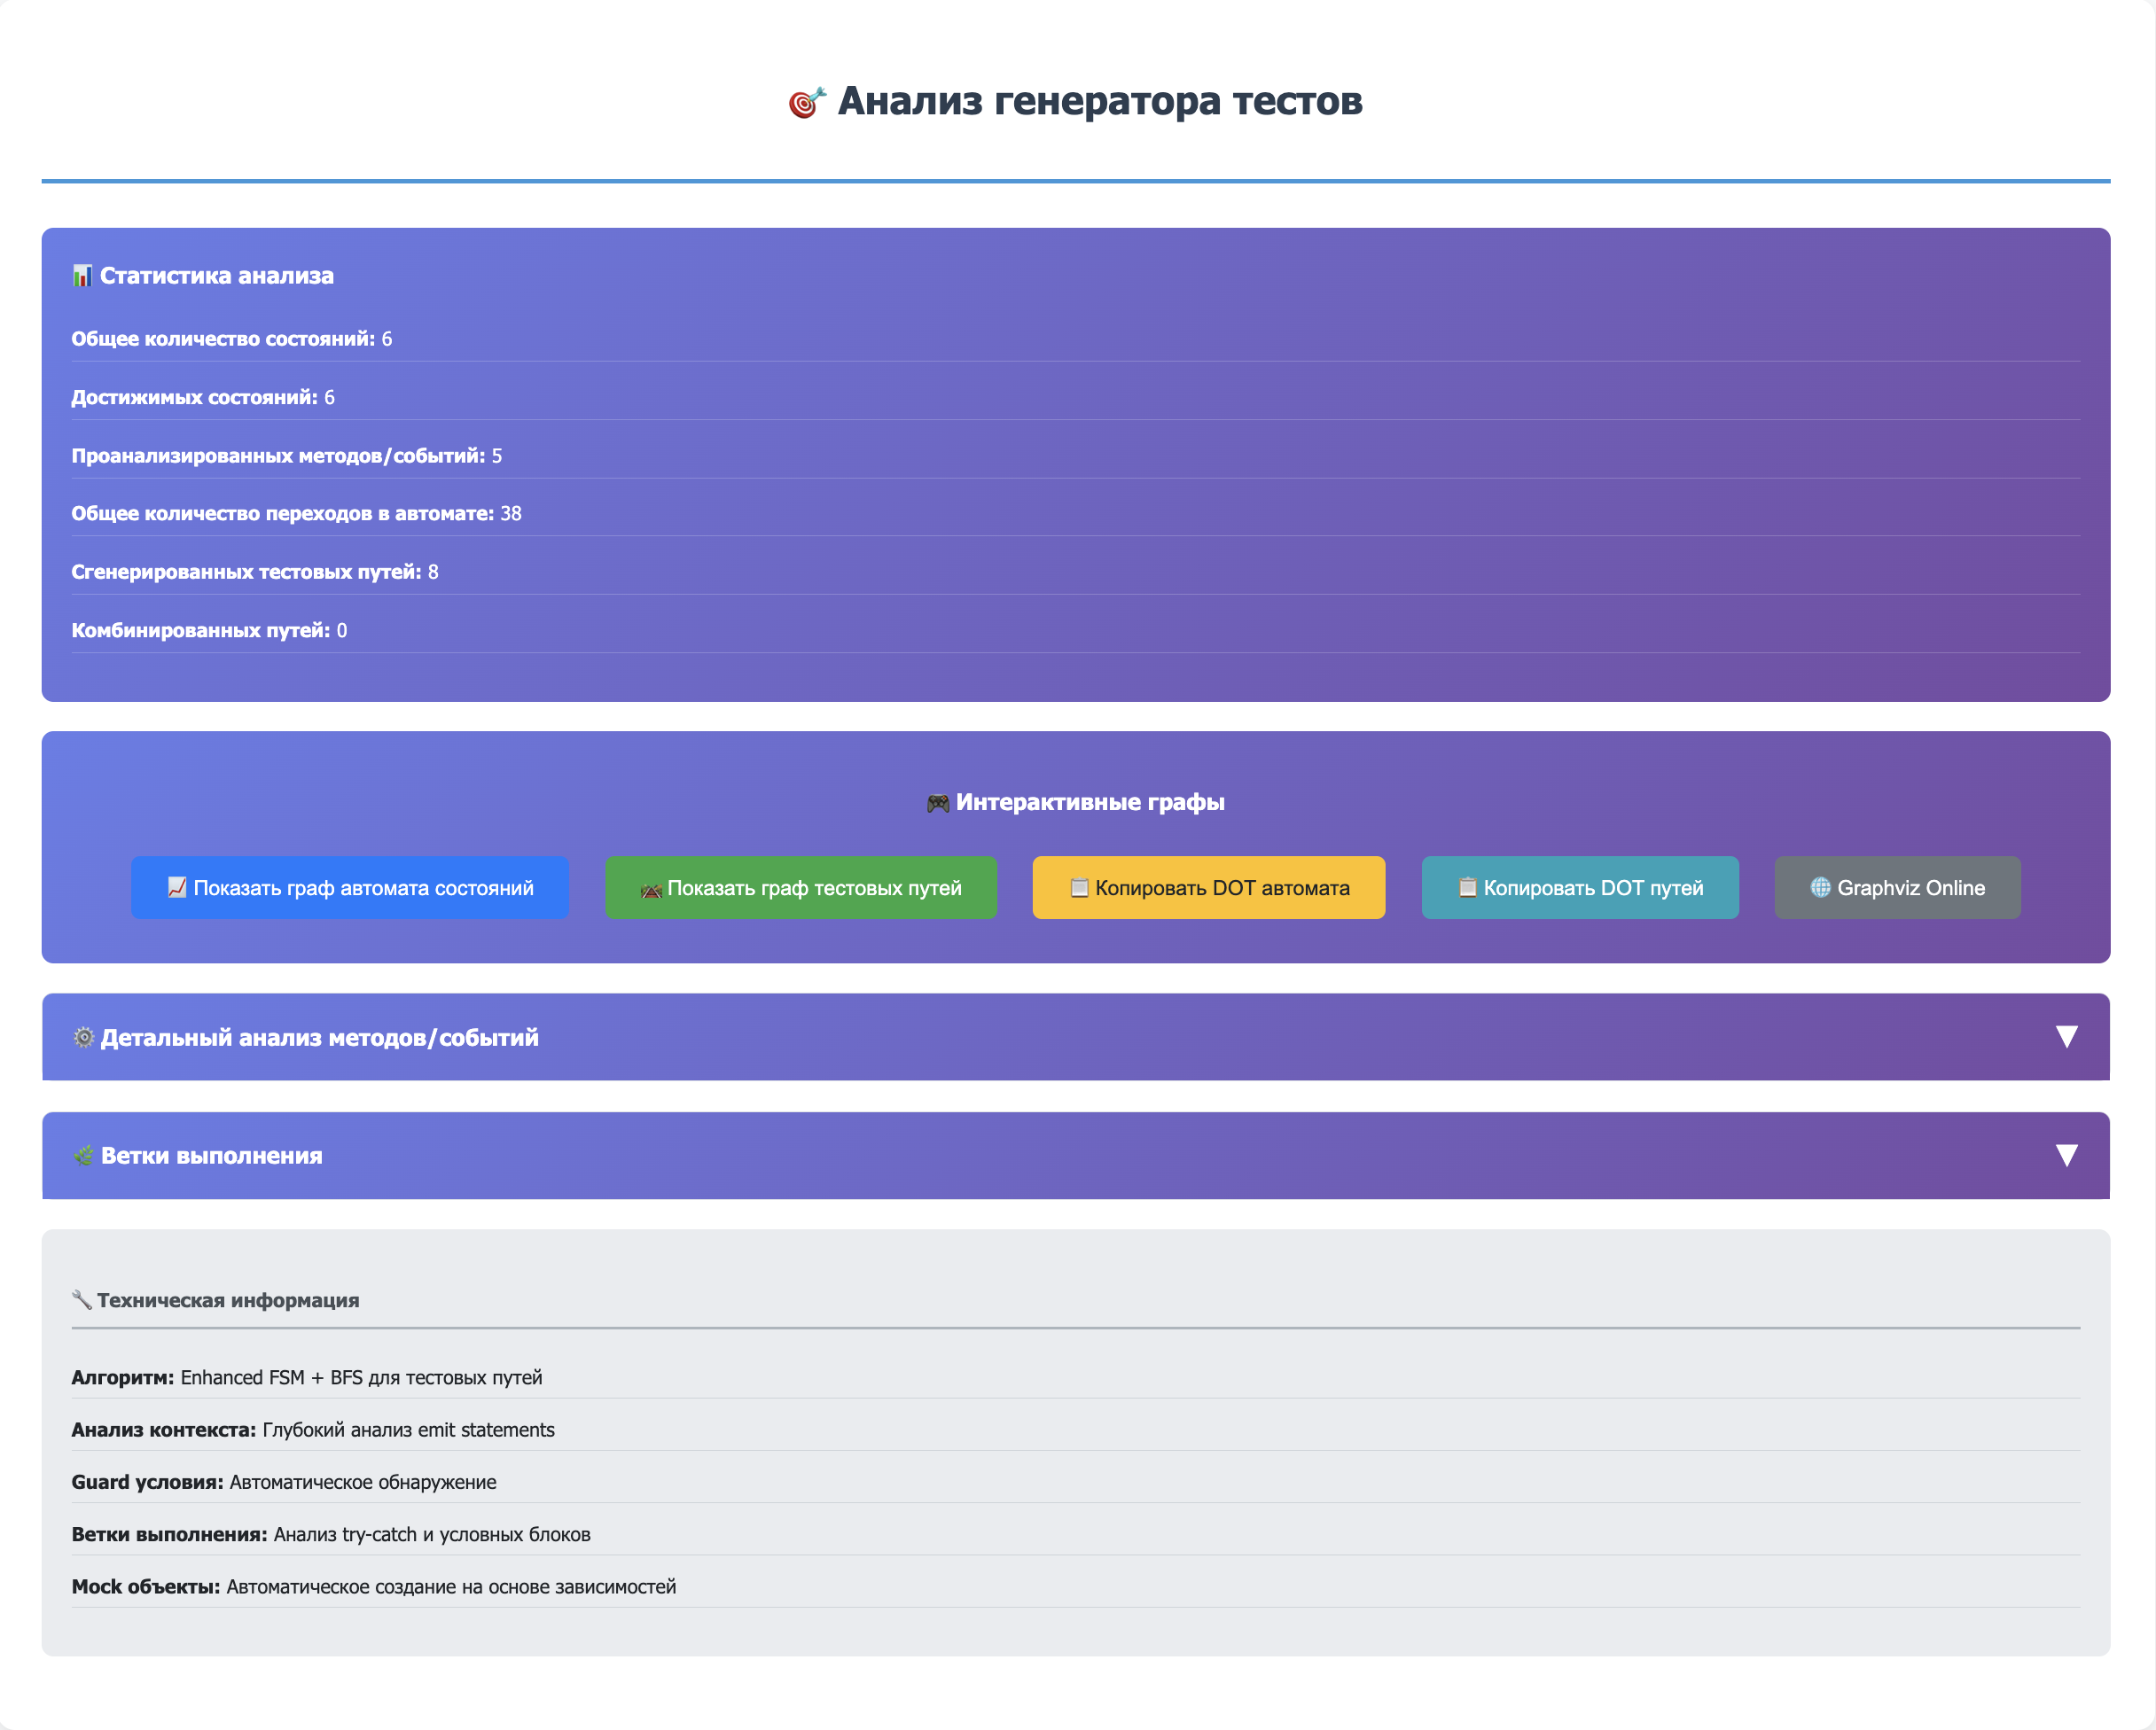
\includegraphics[width=0.8\textwidth]{images/bloc_1.png}
\caption{Общая информация о блоке.}
\label{fig:bloc_info}
\end{figure}

\vspace{2cm}

\begin{figure}[!htb]
\centering
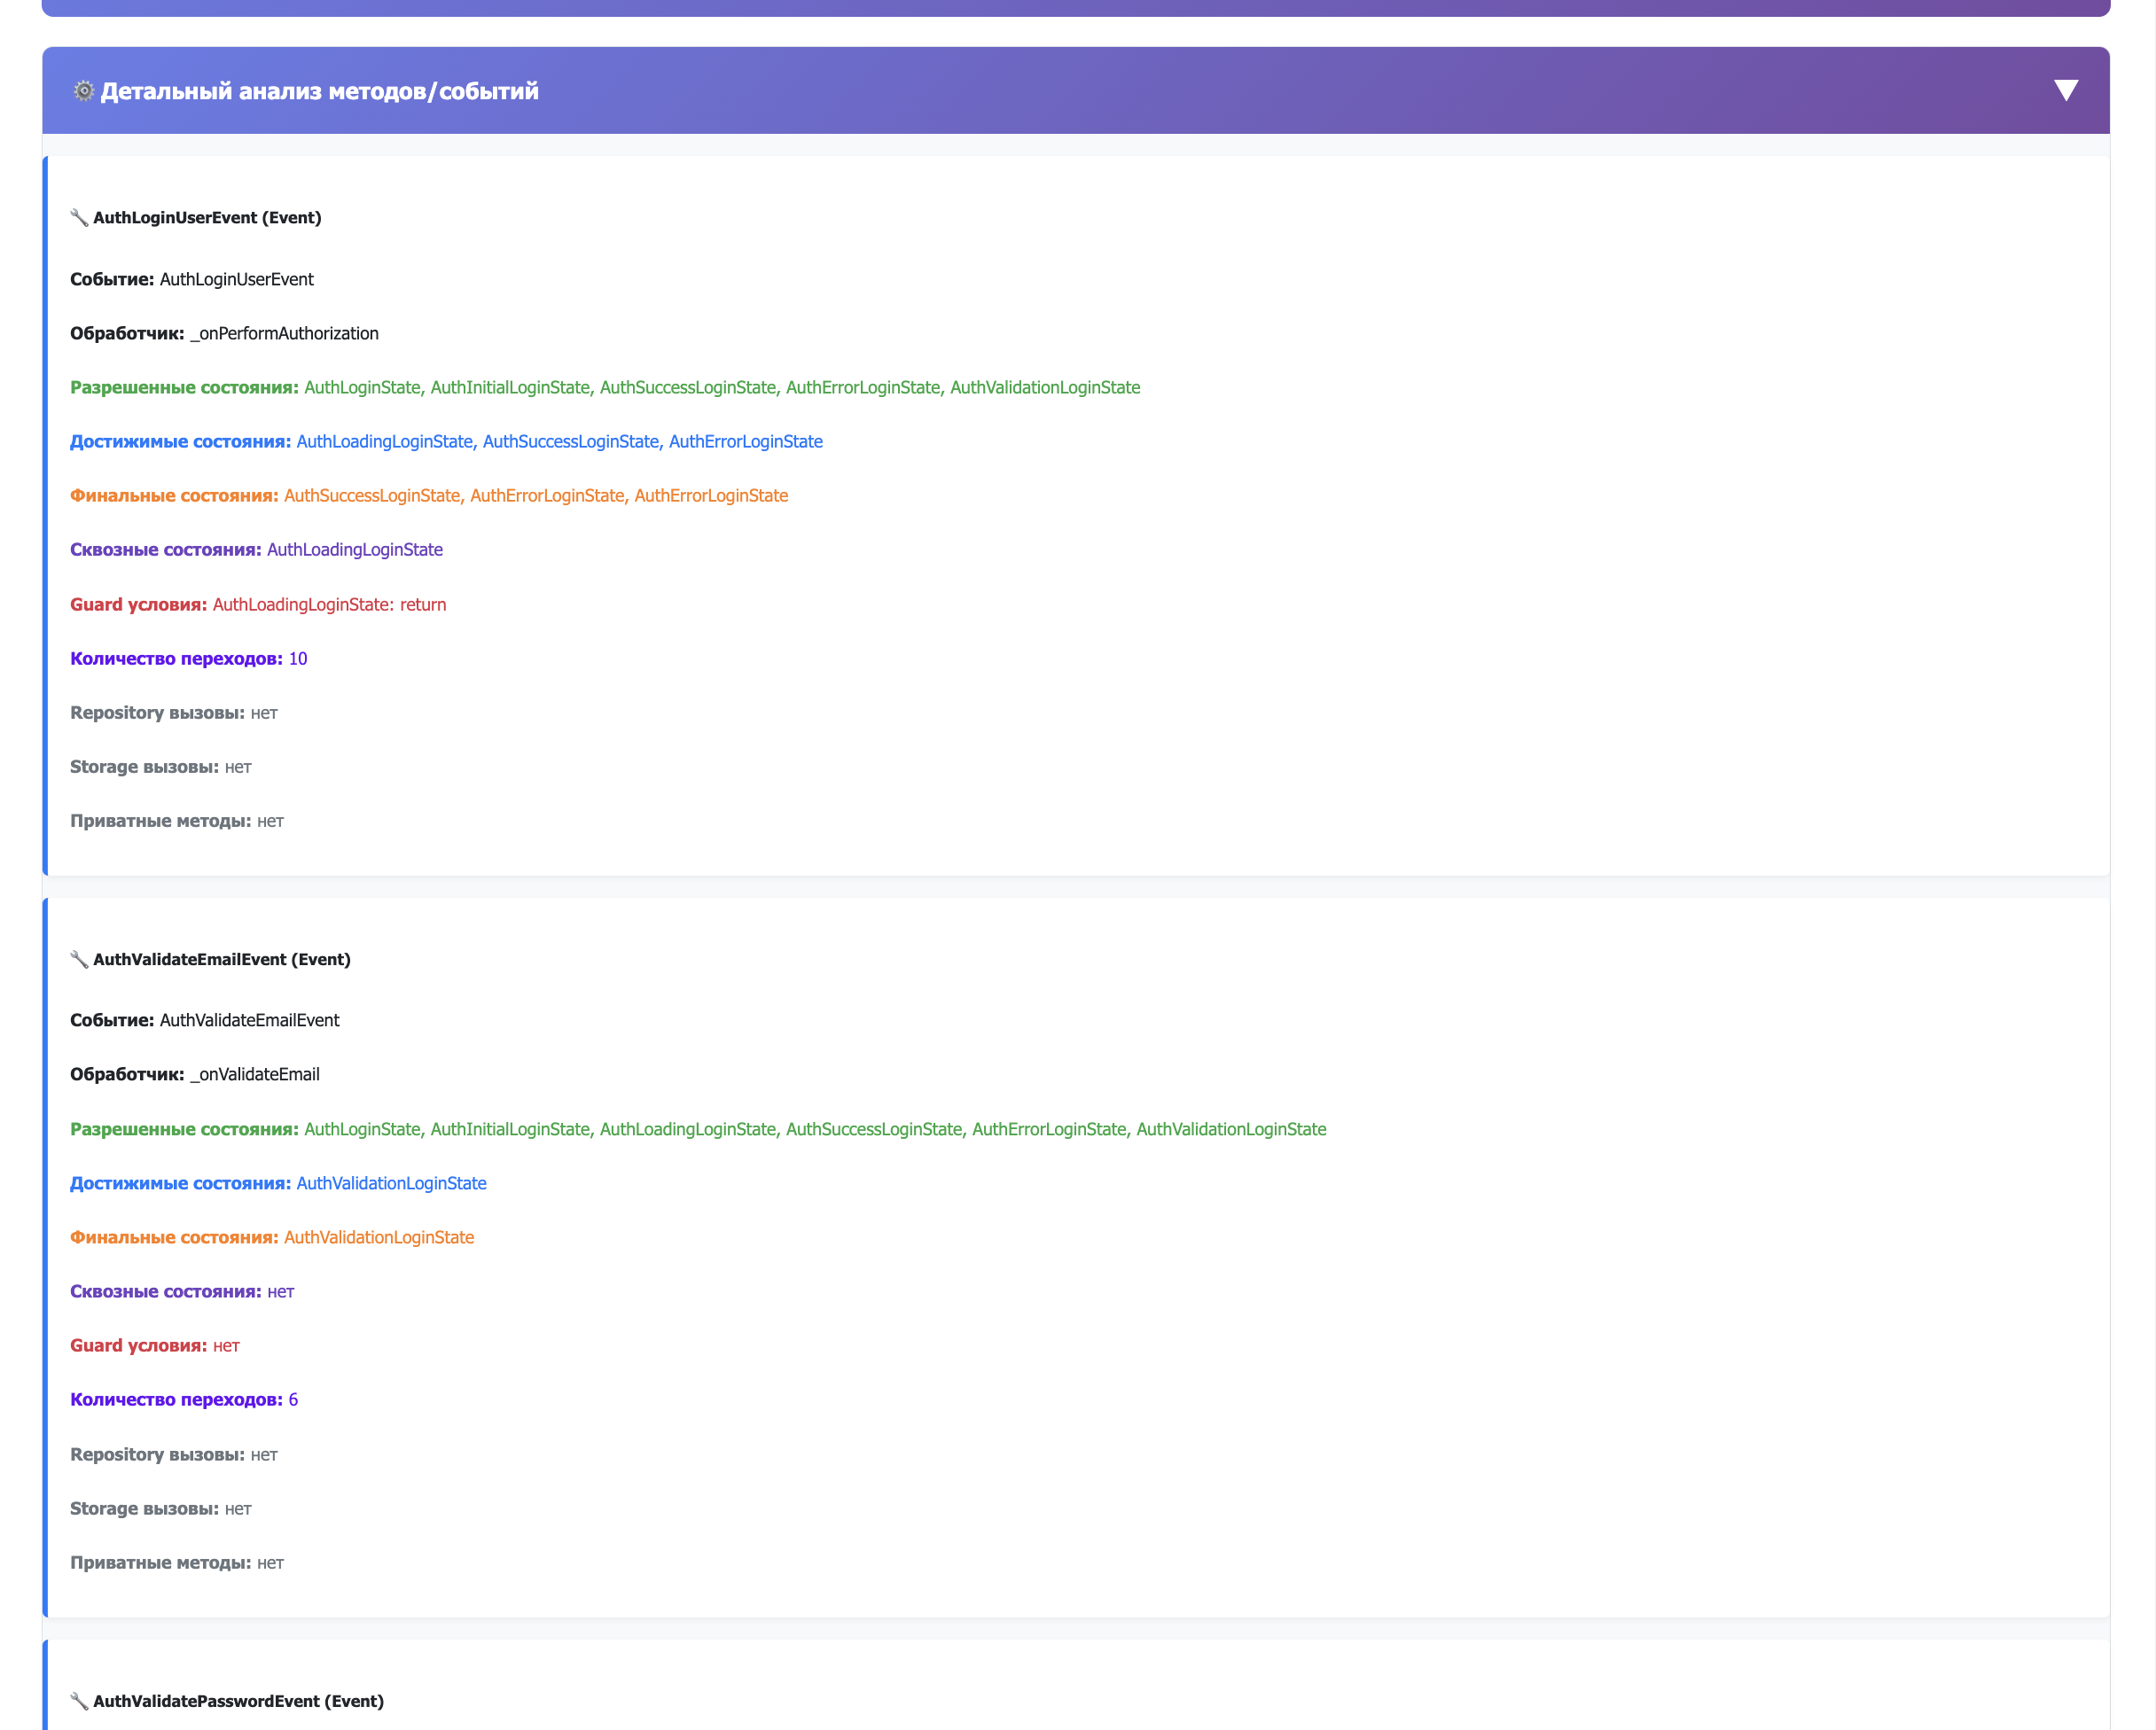
\includegraphics[width=0.7\textwidth]{images/bloc_2.png}
\caption{Информация об ивентах блока.}
\label{fig:bloc_test_info}
\end{figure}

\vspace{2cm}

\begin{figure}[!htb]
\centering
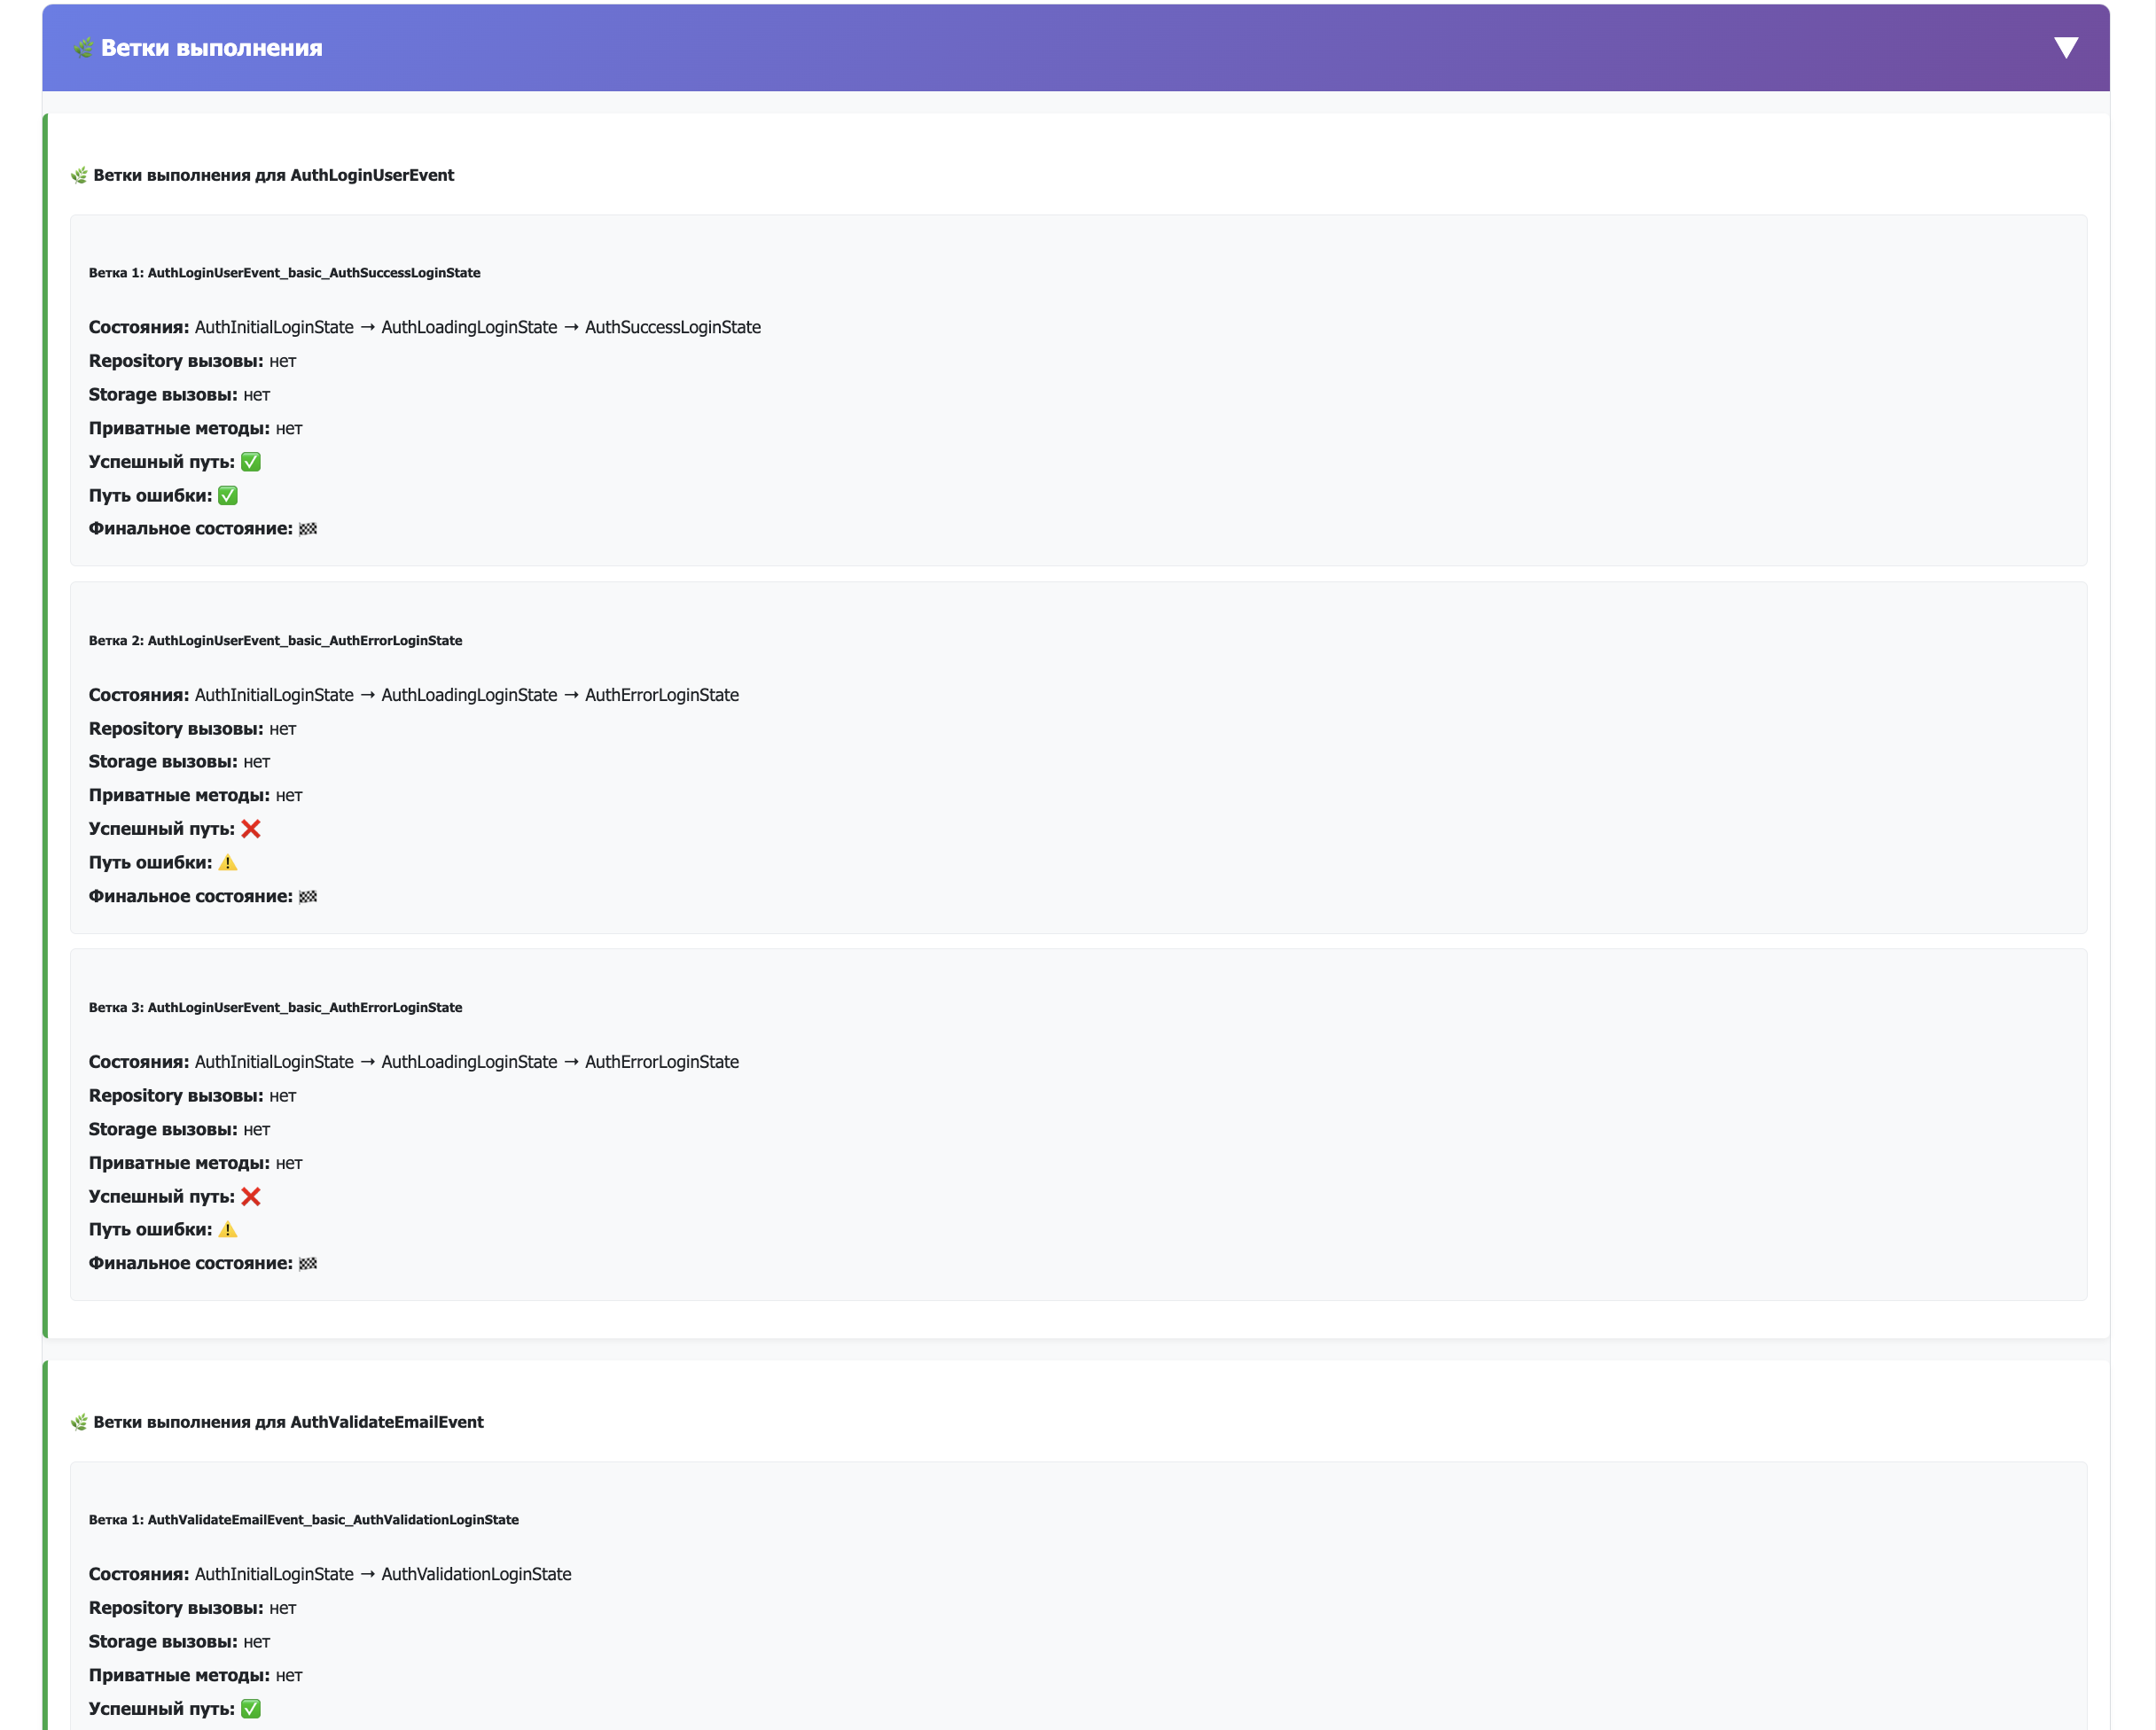
\includegraphics[width=0.8\textwidth]{images/bloc_3.png}
\caption{Информация о тестах блока.}
\label{fig:bloc_automat_1}
\end{figure}

\vspace{2cm}

\begin{figure}[!htb]
\centering
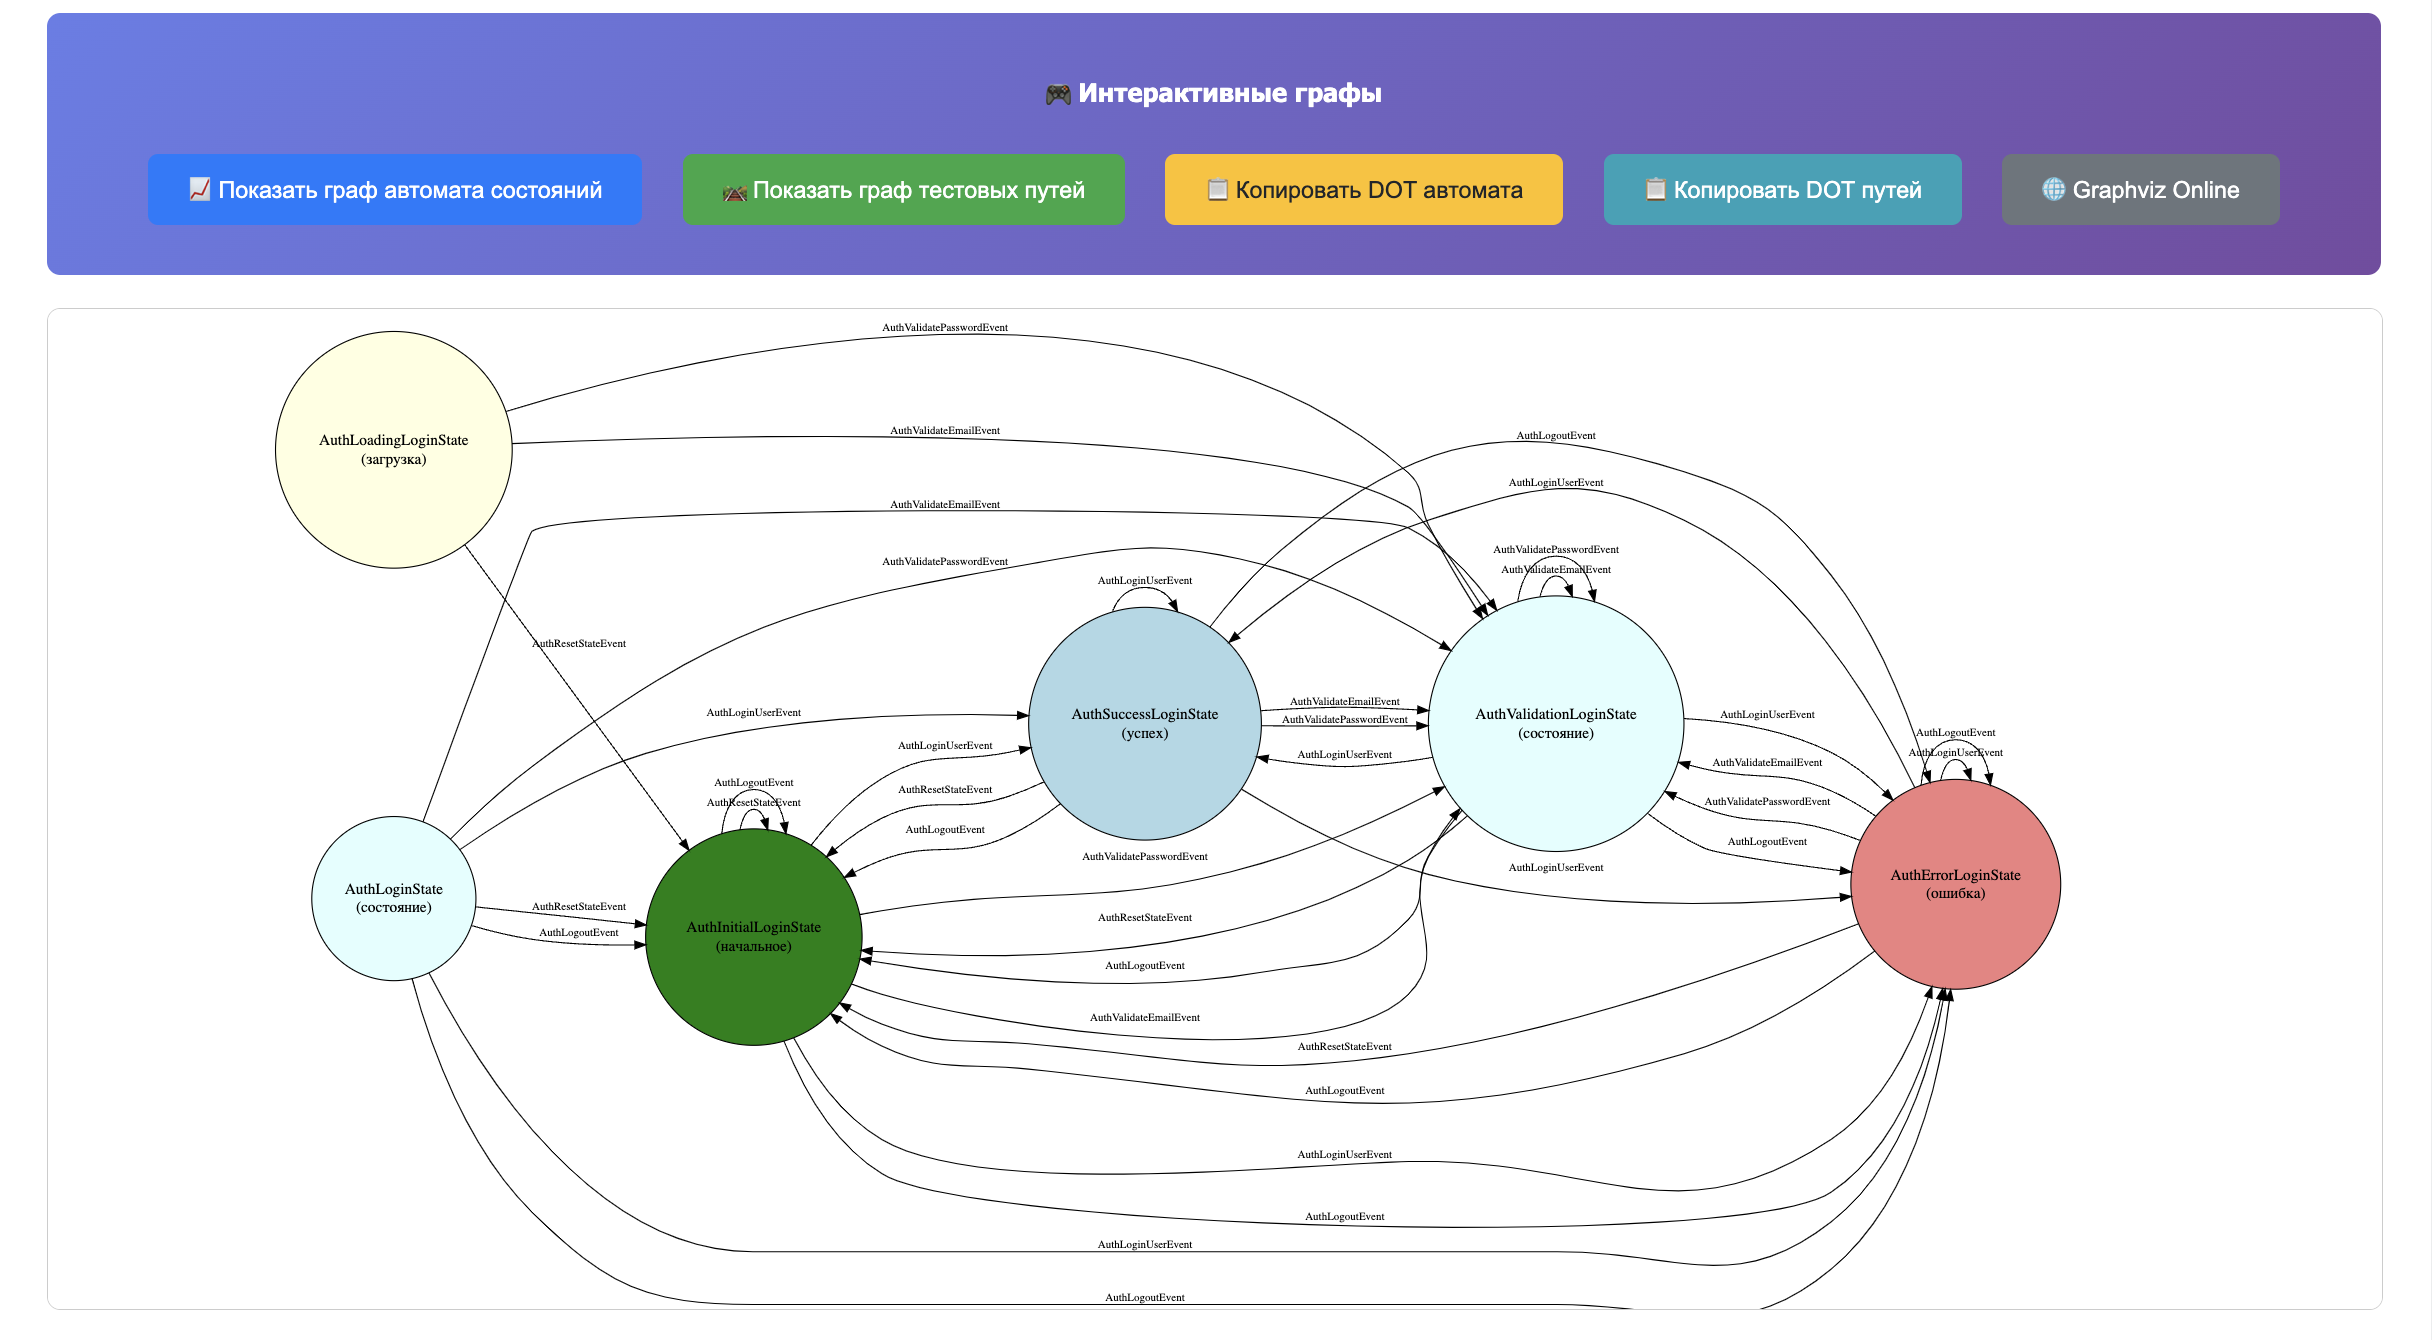
\includegraphics[width=0.7\textwidth]{images/bloc_4.png}
\caption{Атомат состояний блока.}
\label{fig:bloc_automat_2}
\end{figure}

\vspace{2cm}

\begin{figure}[!htb]
\centering
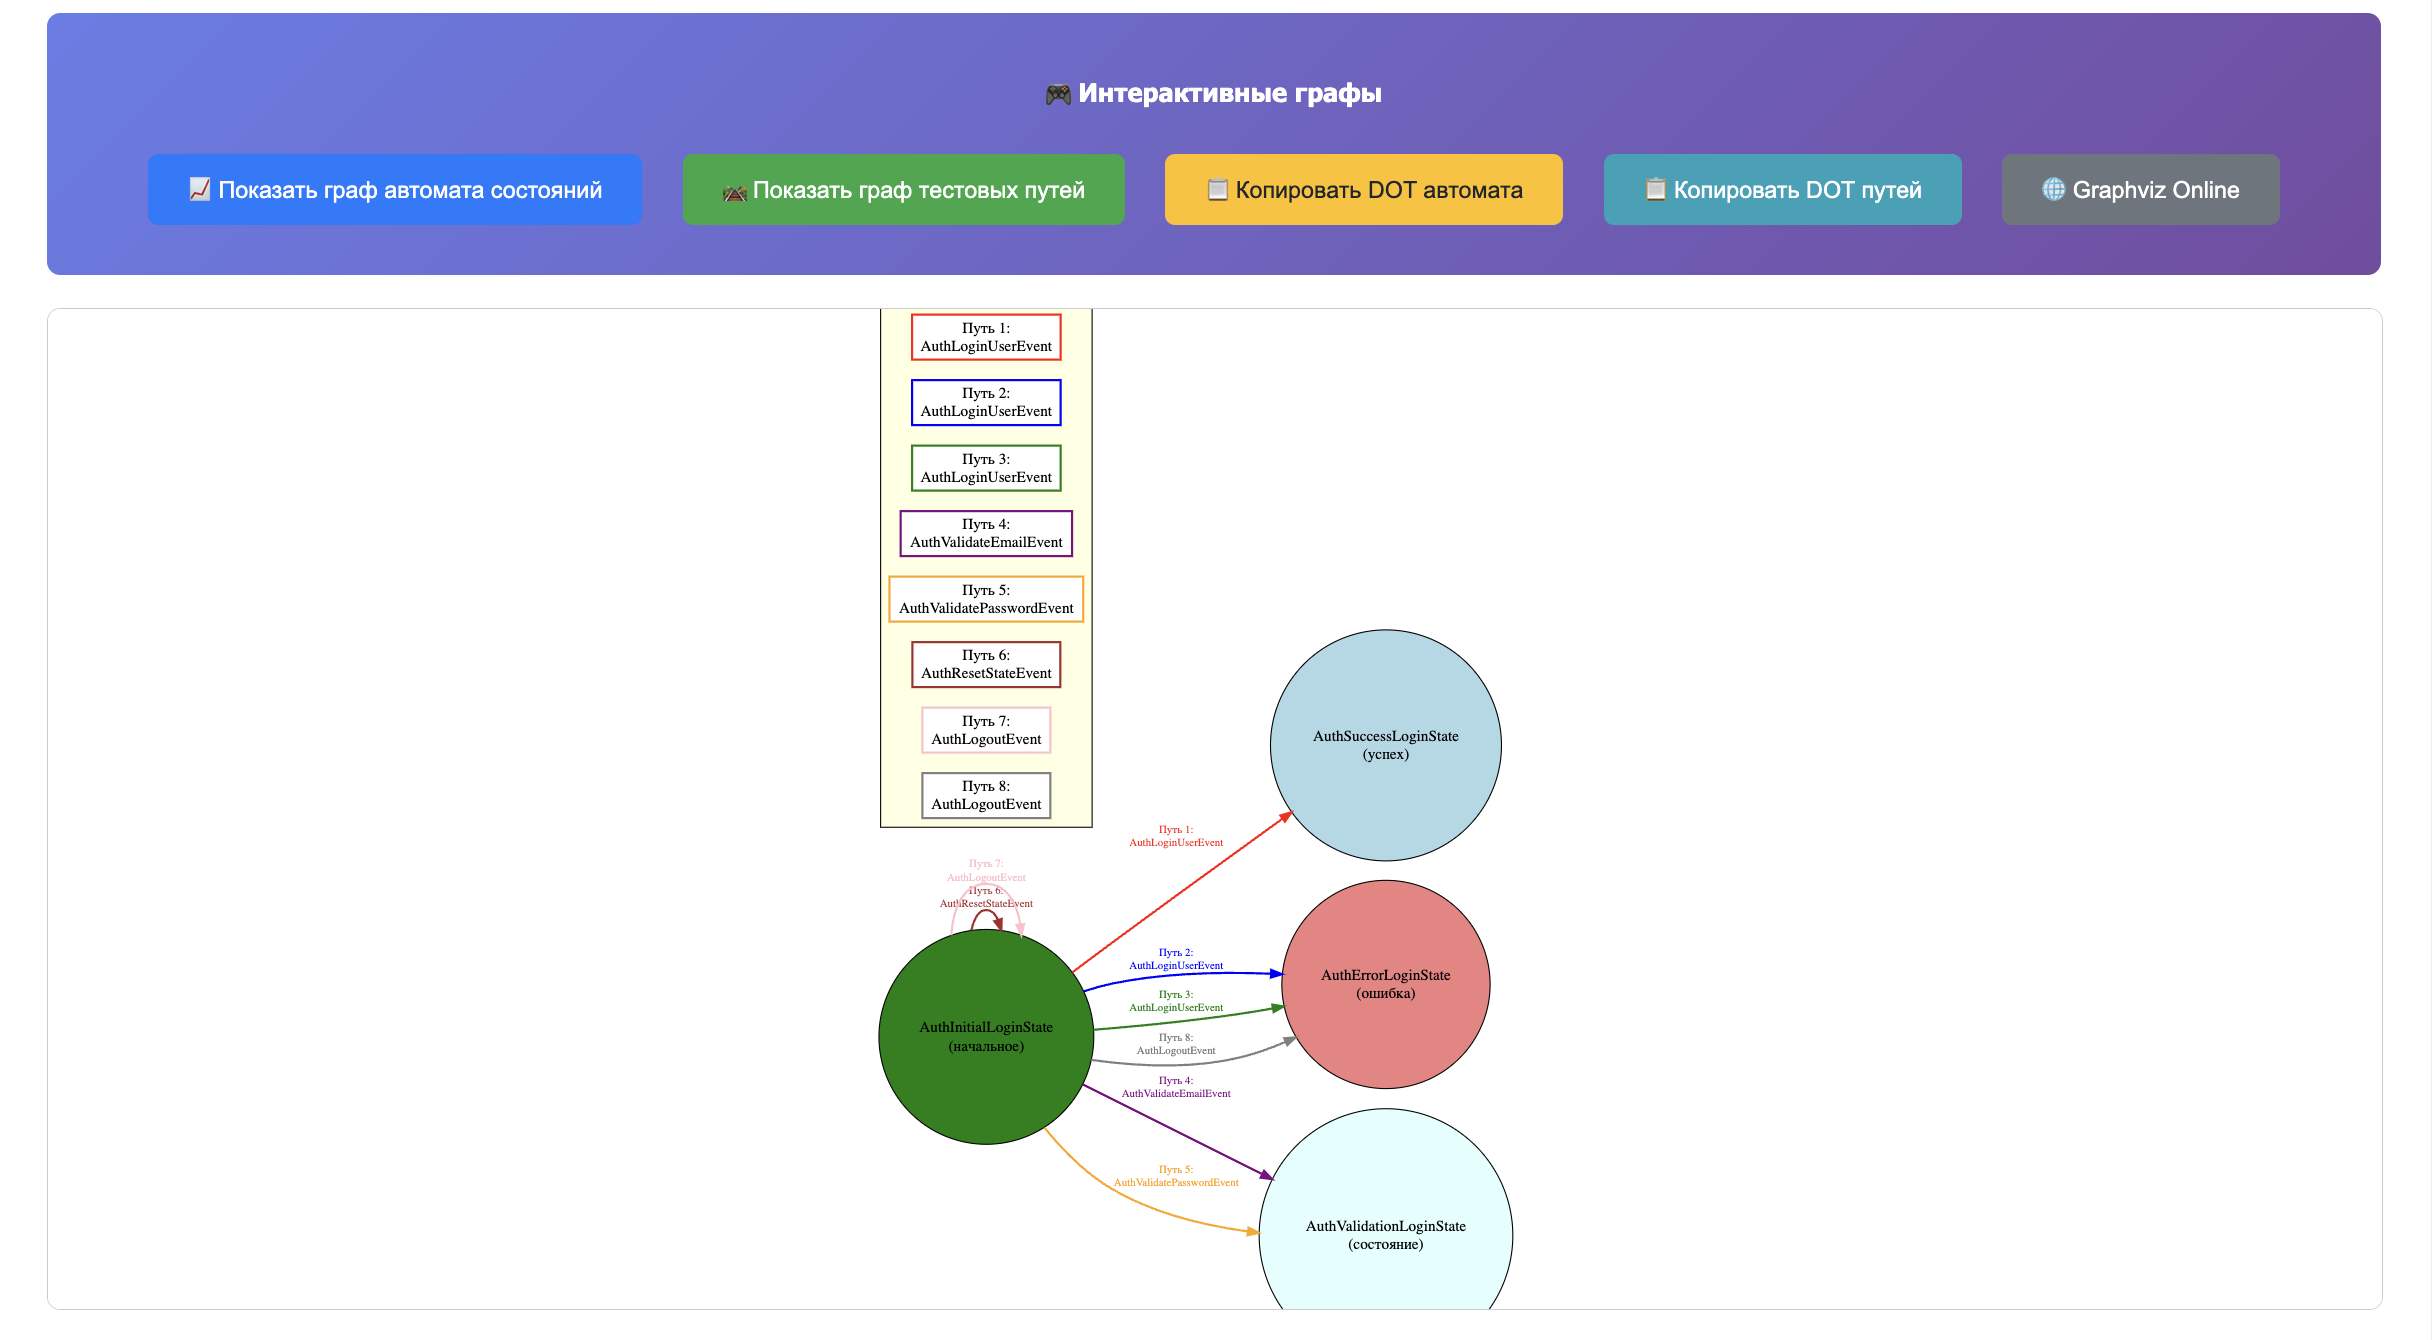
\includegraphics[width=0.7\textwidth]{images/bloc_5.png}
\caption{Тестовые множества блока.}
\label{fig:bloc_more_info}
\end{figure}

% ================== ПРИЛОЖЕНИЕ Б: ВЫПОЛНЕНИЕ ПРОГРАММЫ ДЛЯ КУБИТА ==================
\newpage
\anonsection{ПРИЛОЖЕНИЕ Б}

В данном приложении представлены изображения генеративного информационного файла, при вызове генерации тестов для \texttt{notification\_toggle\_cubit}.

\begin{figure}[!htb]
\centering
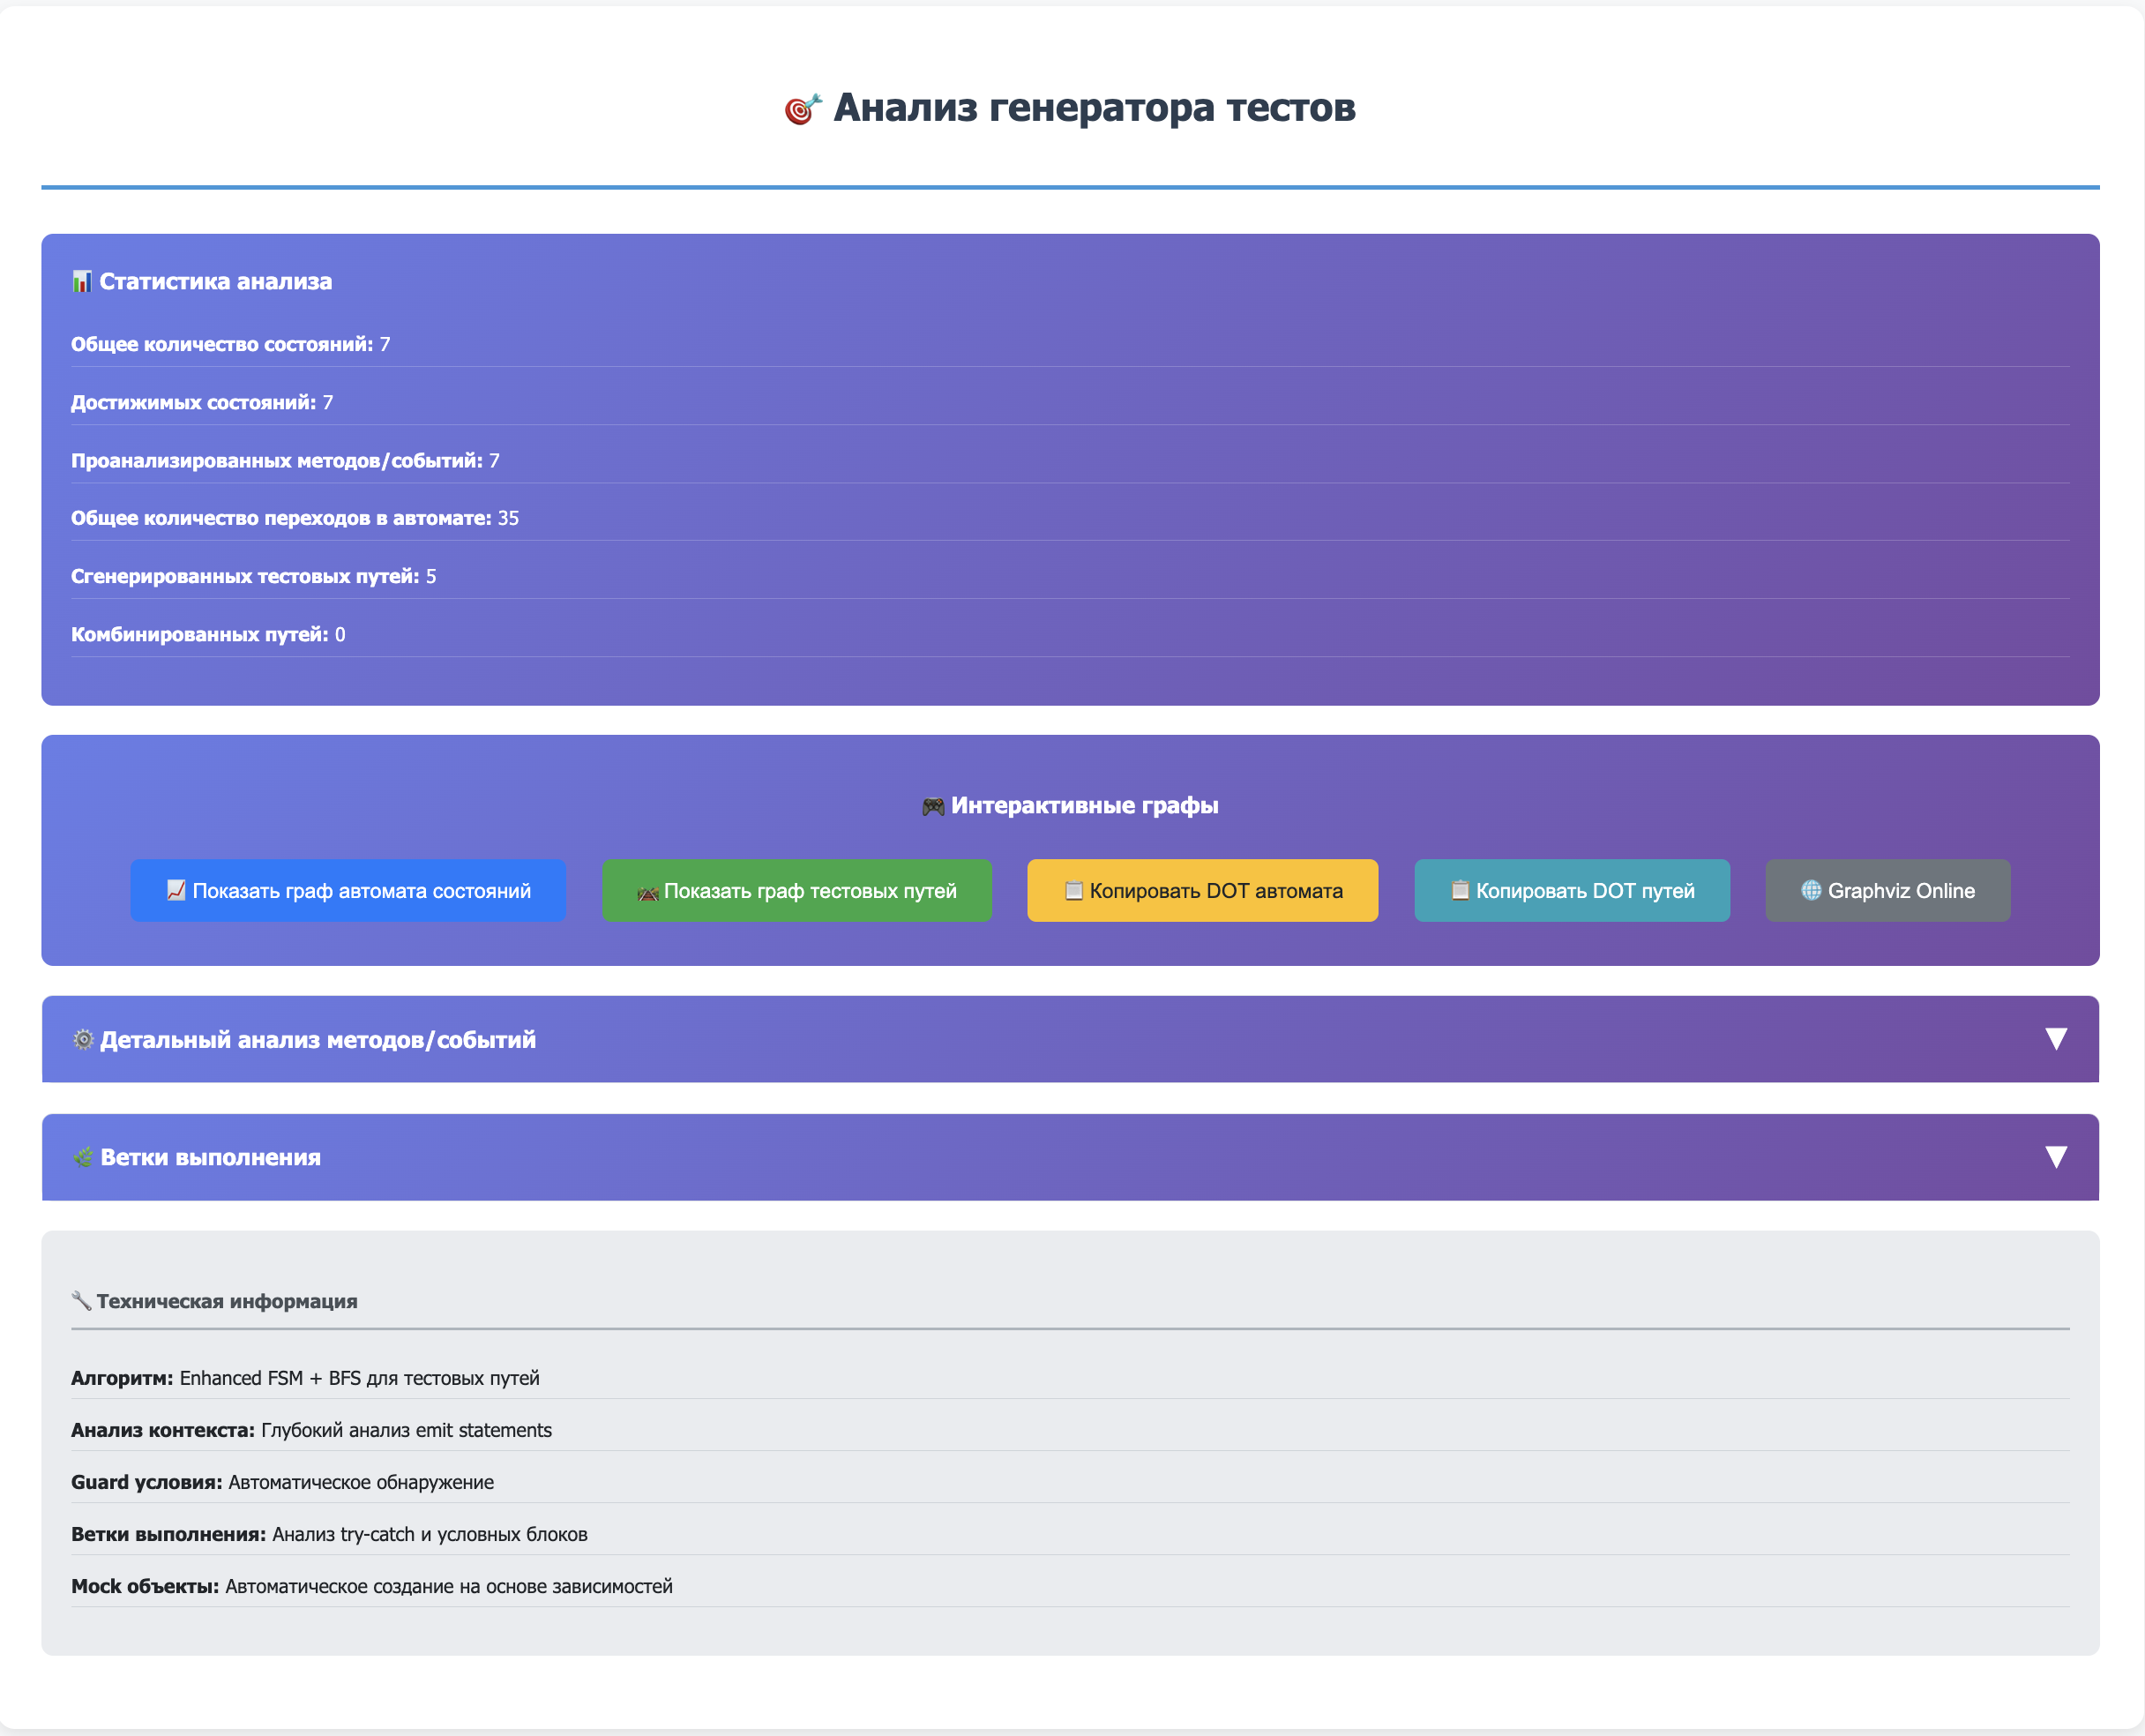
\includegraphics[width=0.8\textwidth]{images/cubit_1.png}
\caption{Общая информация о кубите.}
\label{fig:cubit_info}
\end{figure}

\vspace{2cm}

\begin{figure}[!htb]
\centering
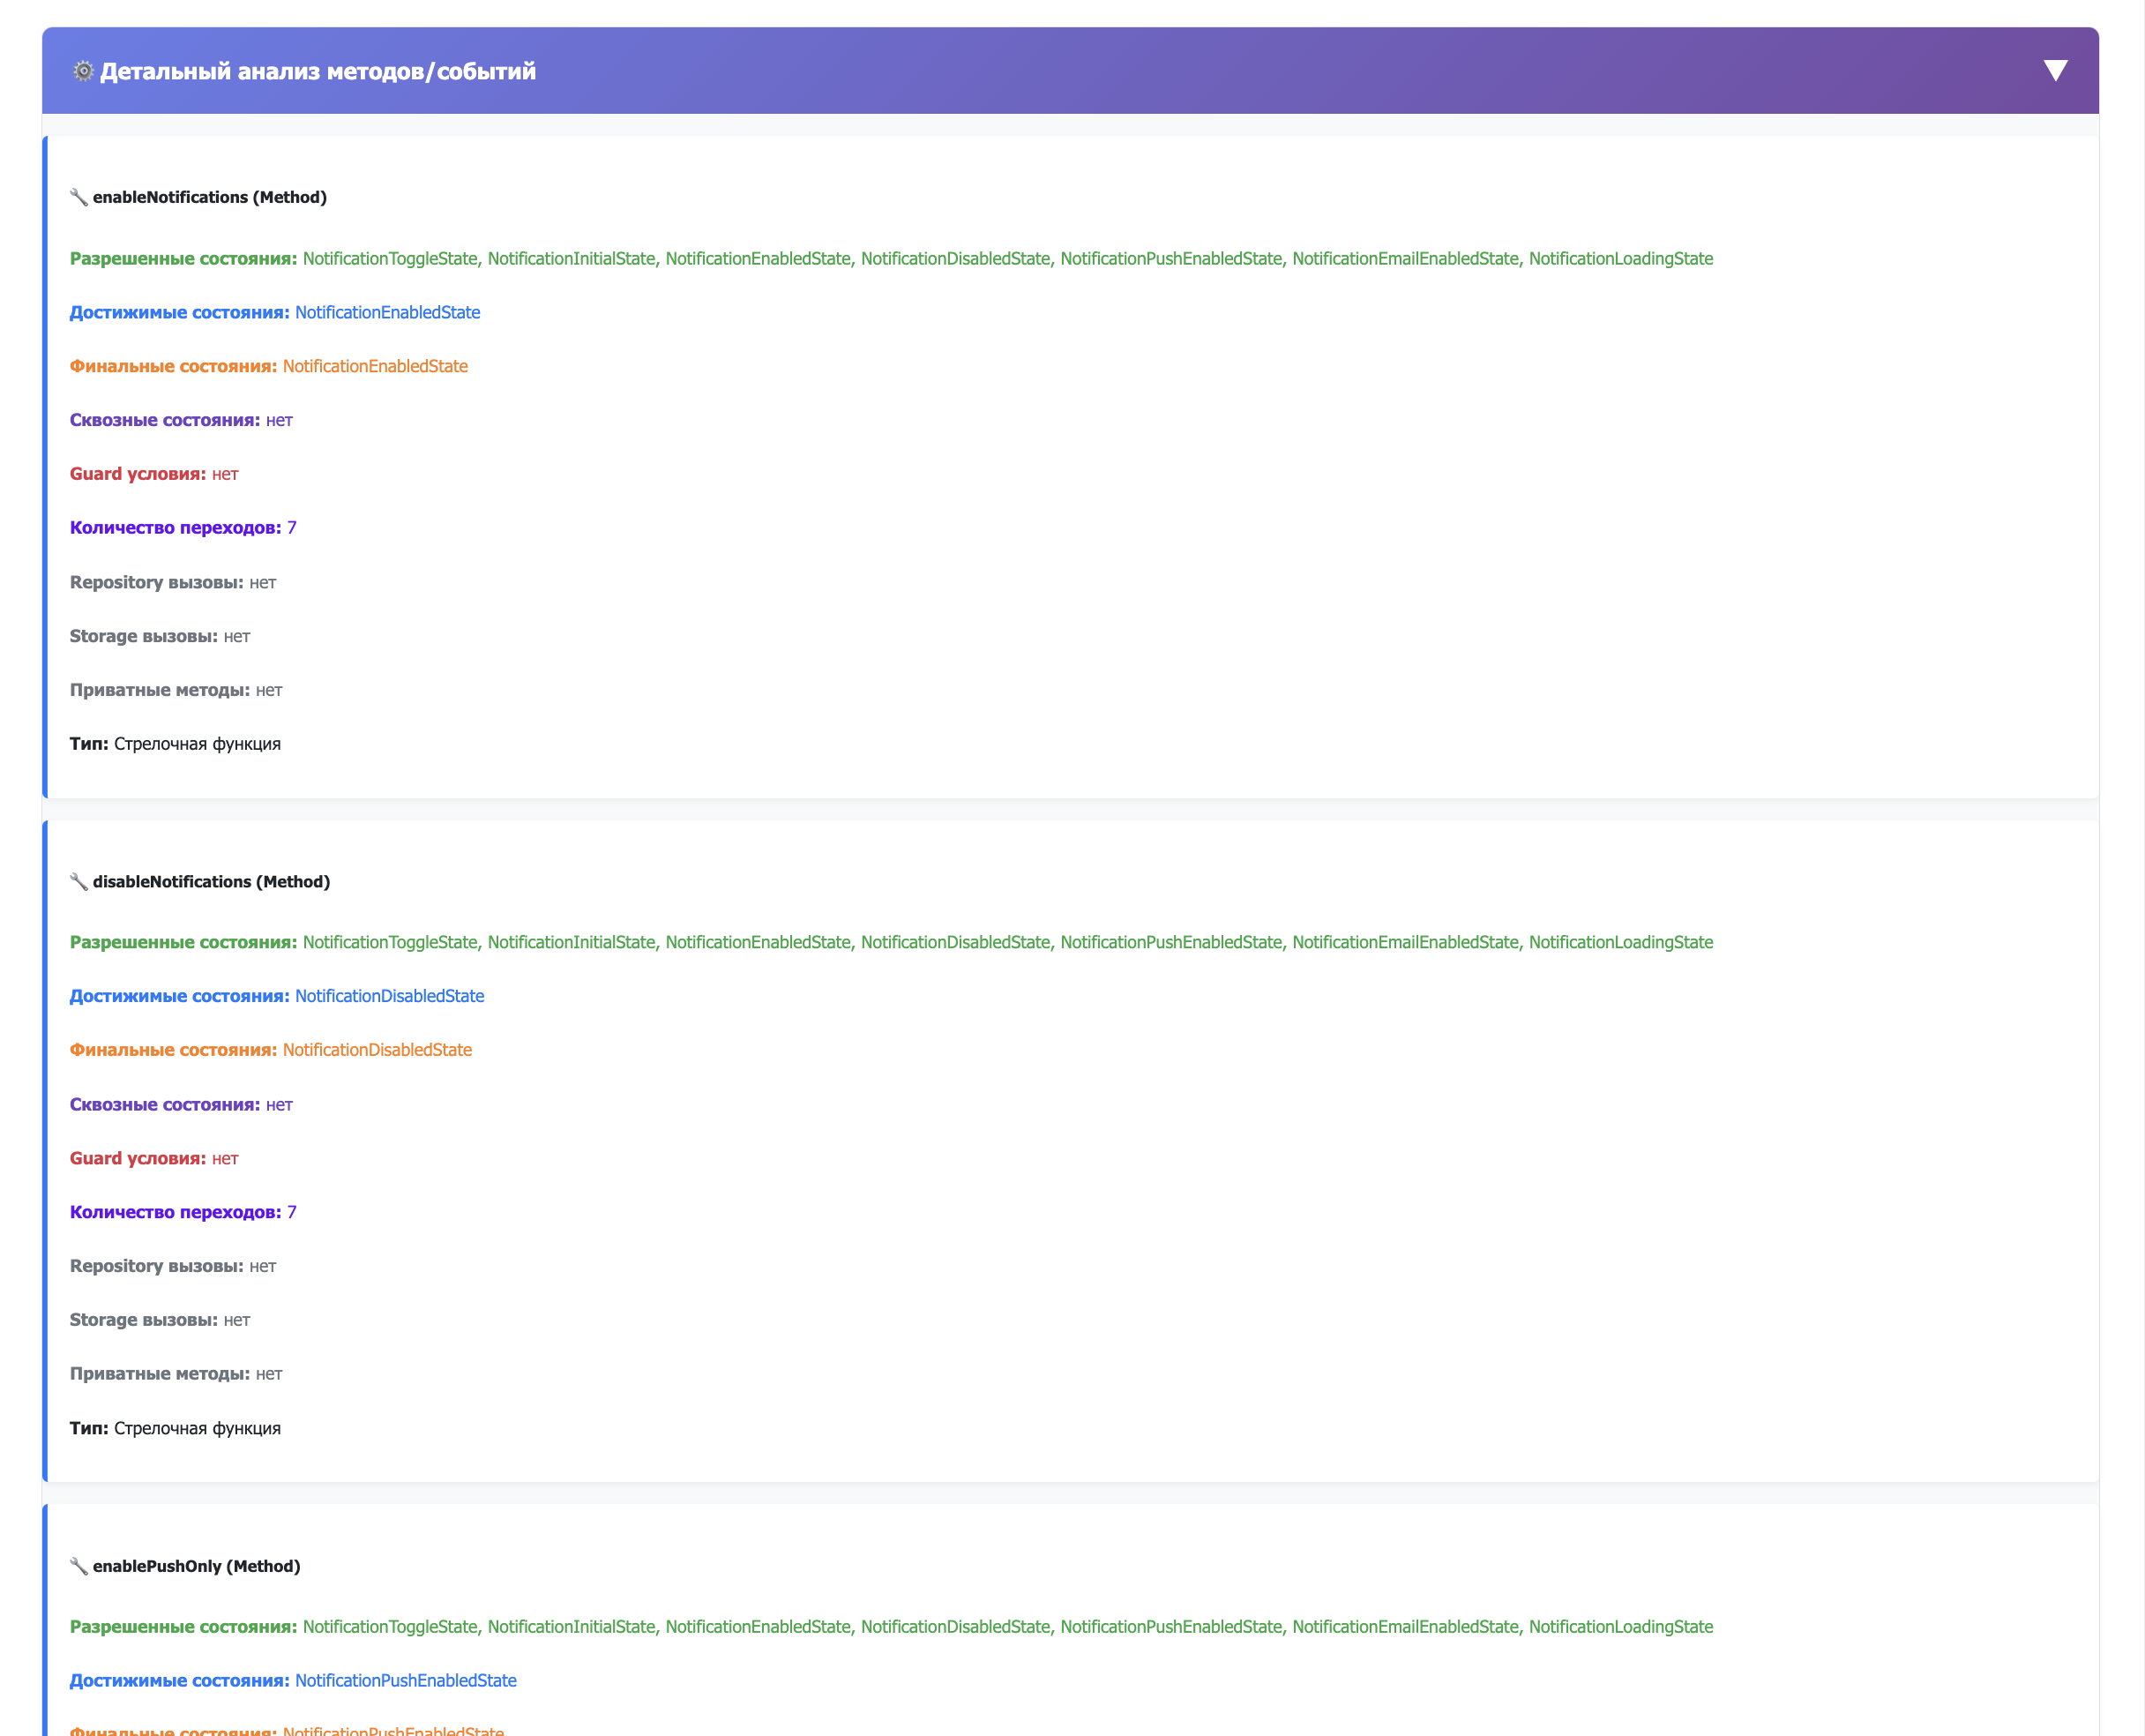
\includegraphics[width=0.7\textwidth]{images/cubit_2.png}
\caption{Информация о методах кубита.}
\label{fig:cubit_test_info}
\end{figure}

\vspace{2cm}

\begin{figure}[!htb]
\centering
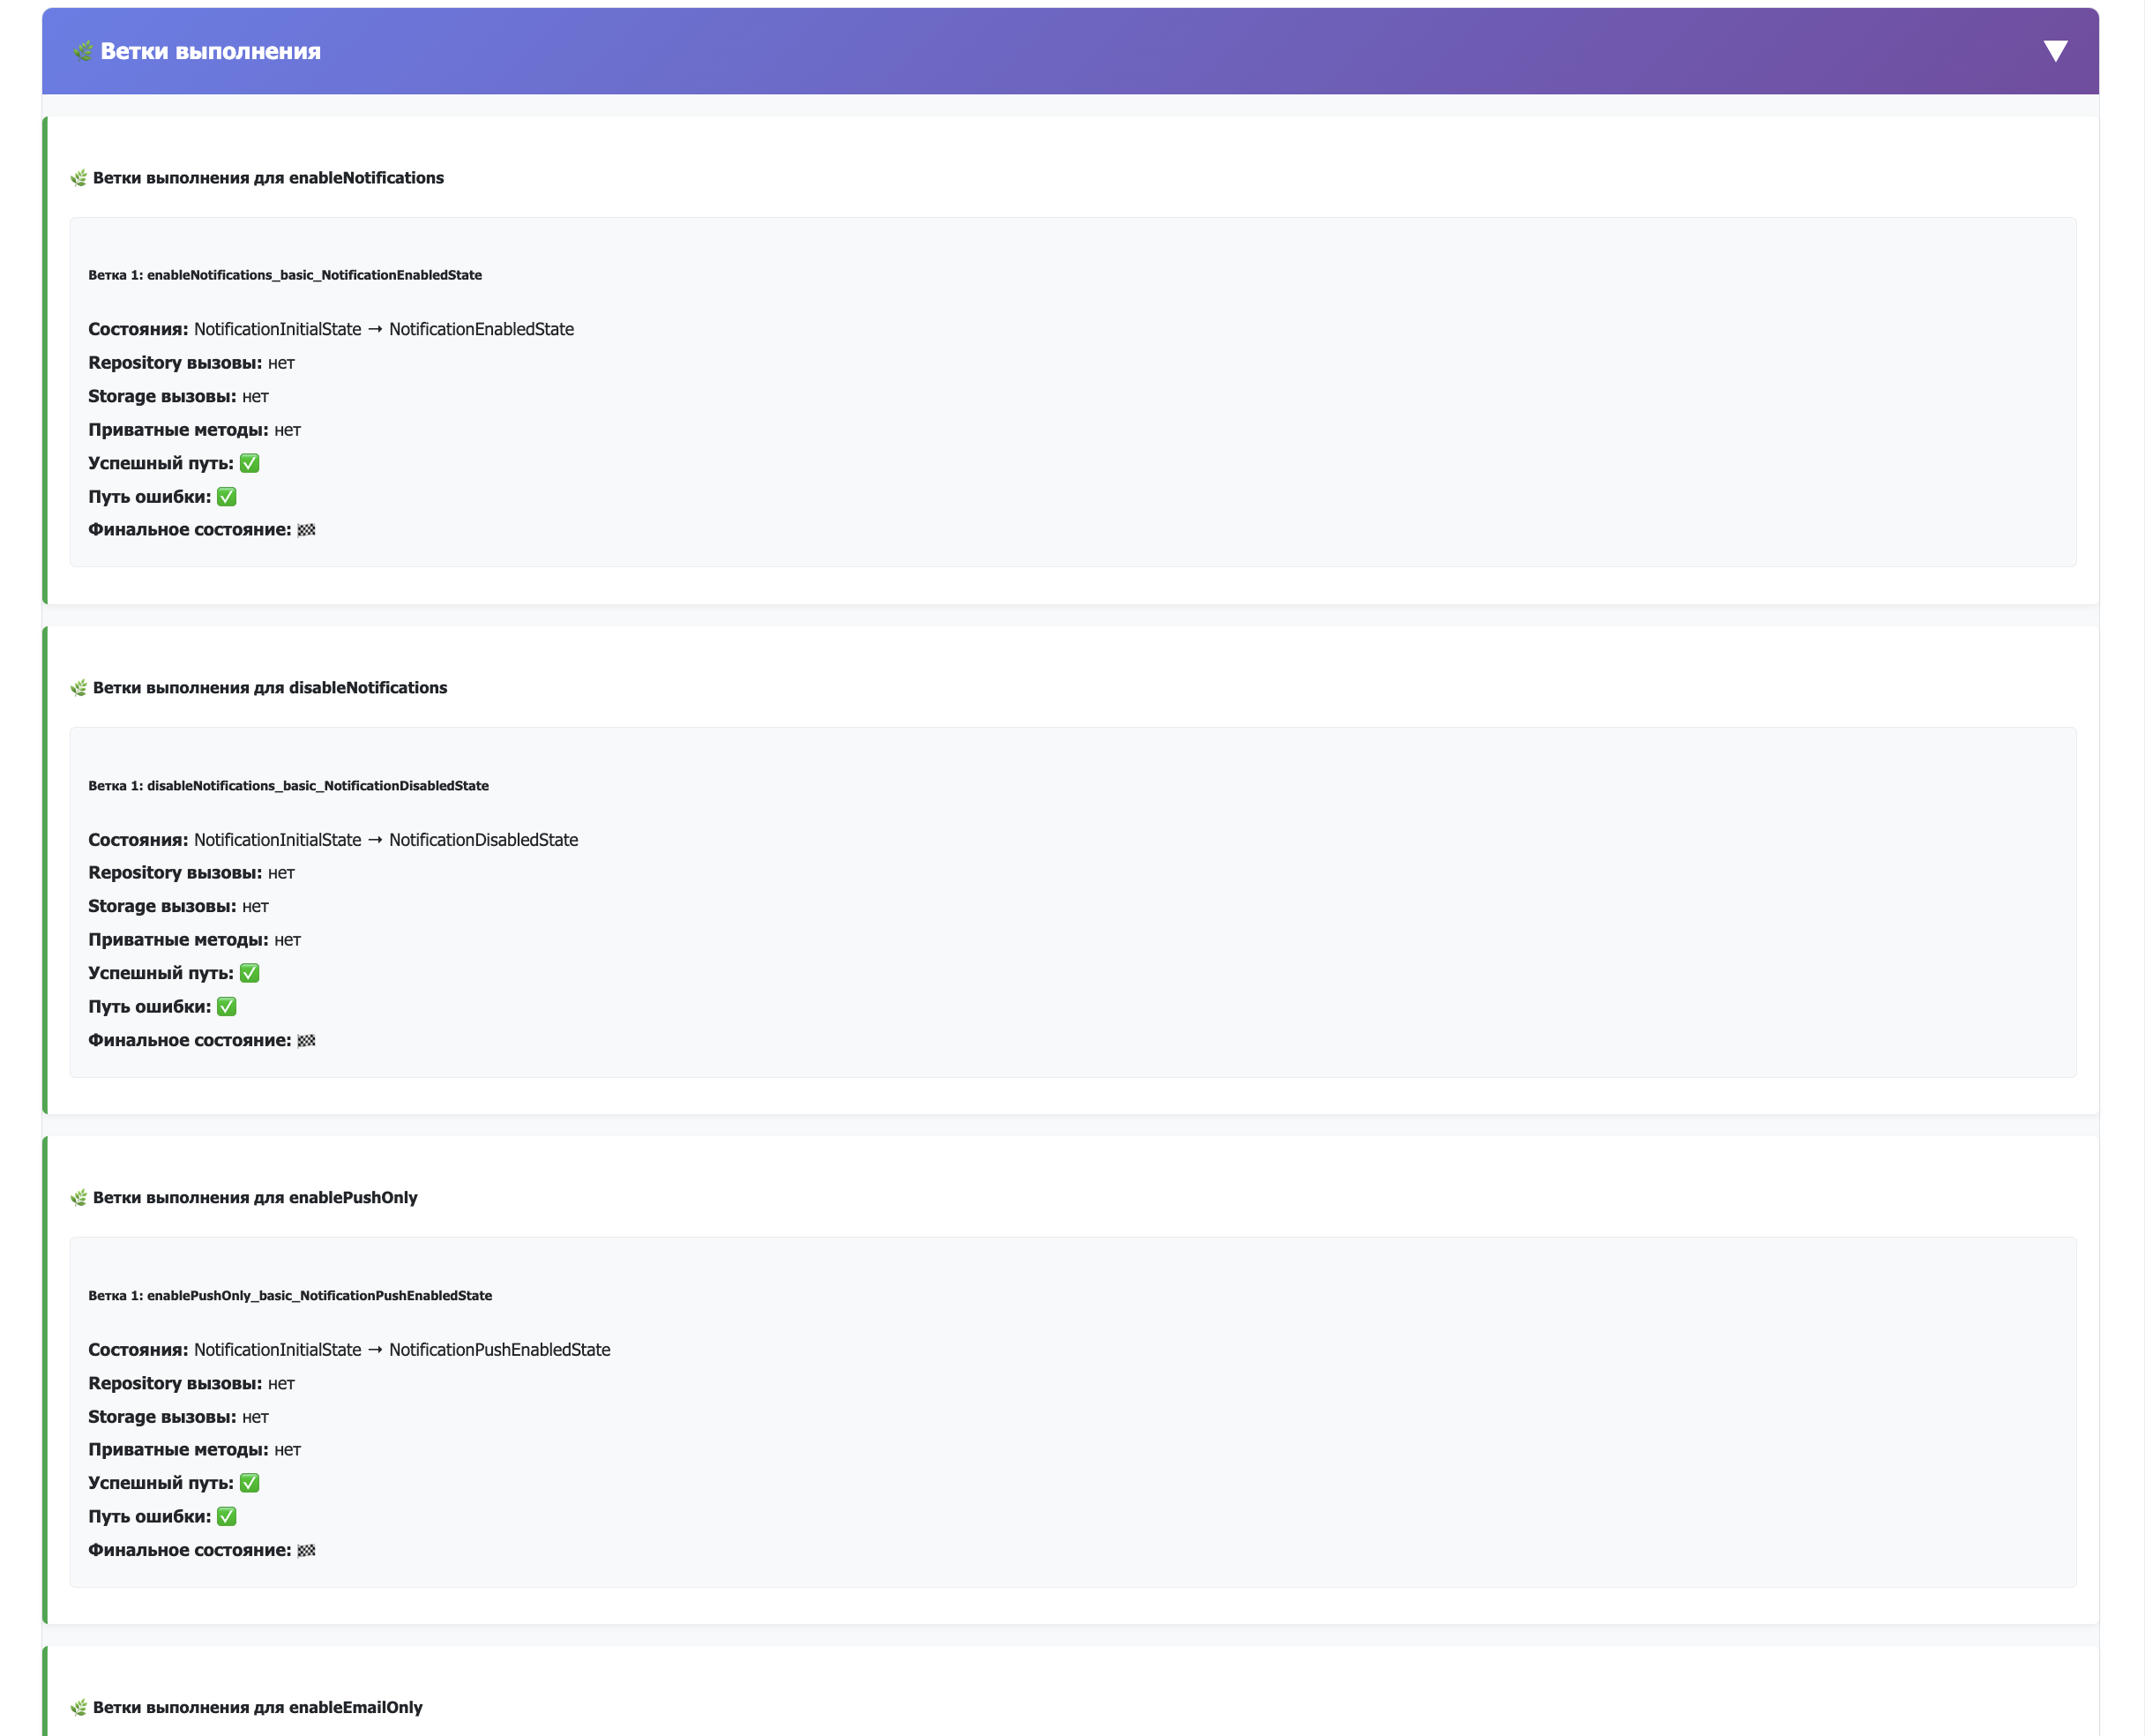
\includegraphics[width=0.8\textwidth]{images/cubit_3.png}
\caption{Информация о тестах кубита.}
\label{fig:cubit_automat}
\end{figure}

\vspace{2cm}

\begin{figure}[!htb]
\centering
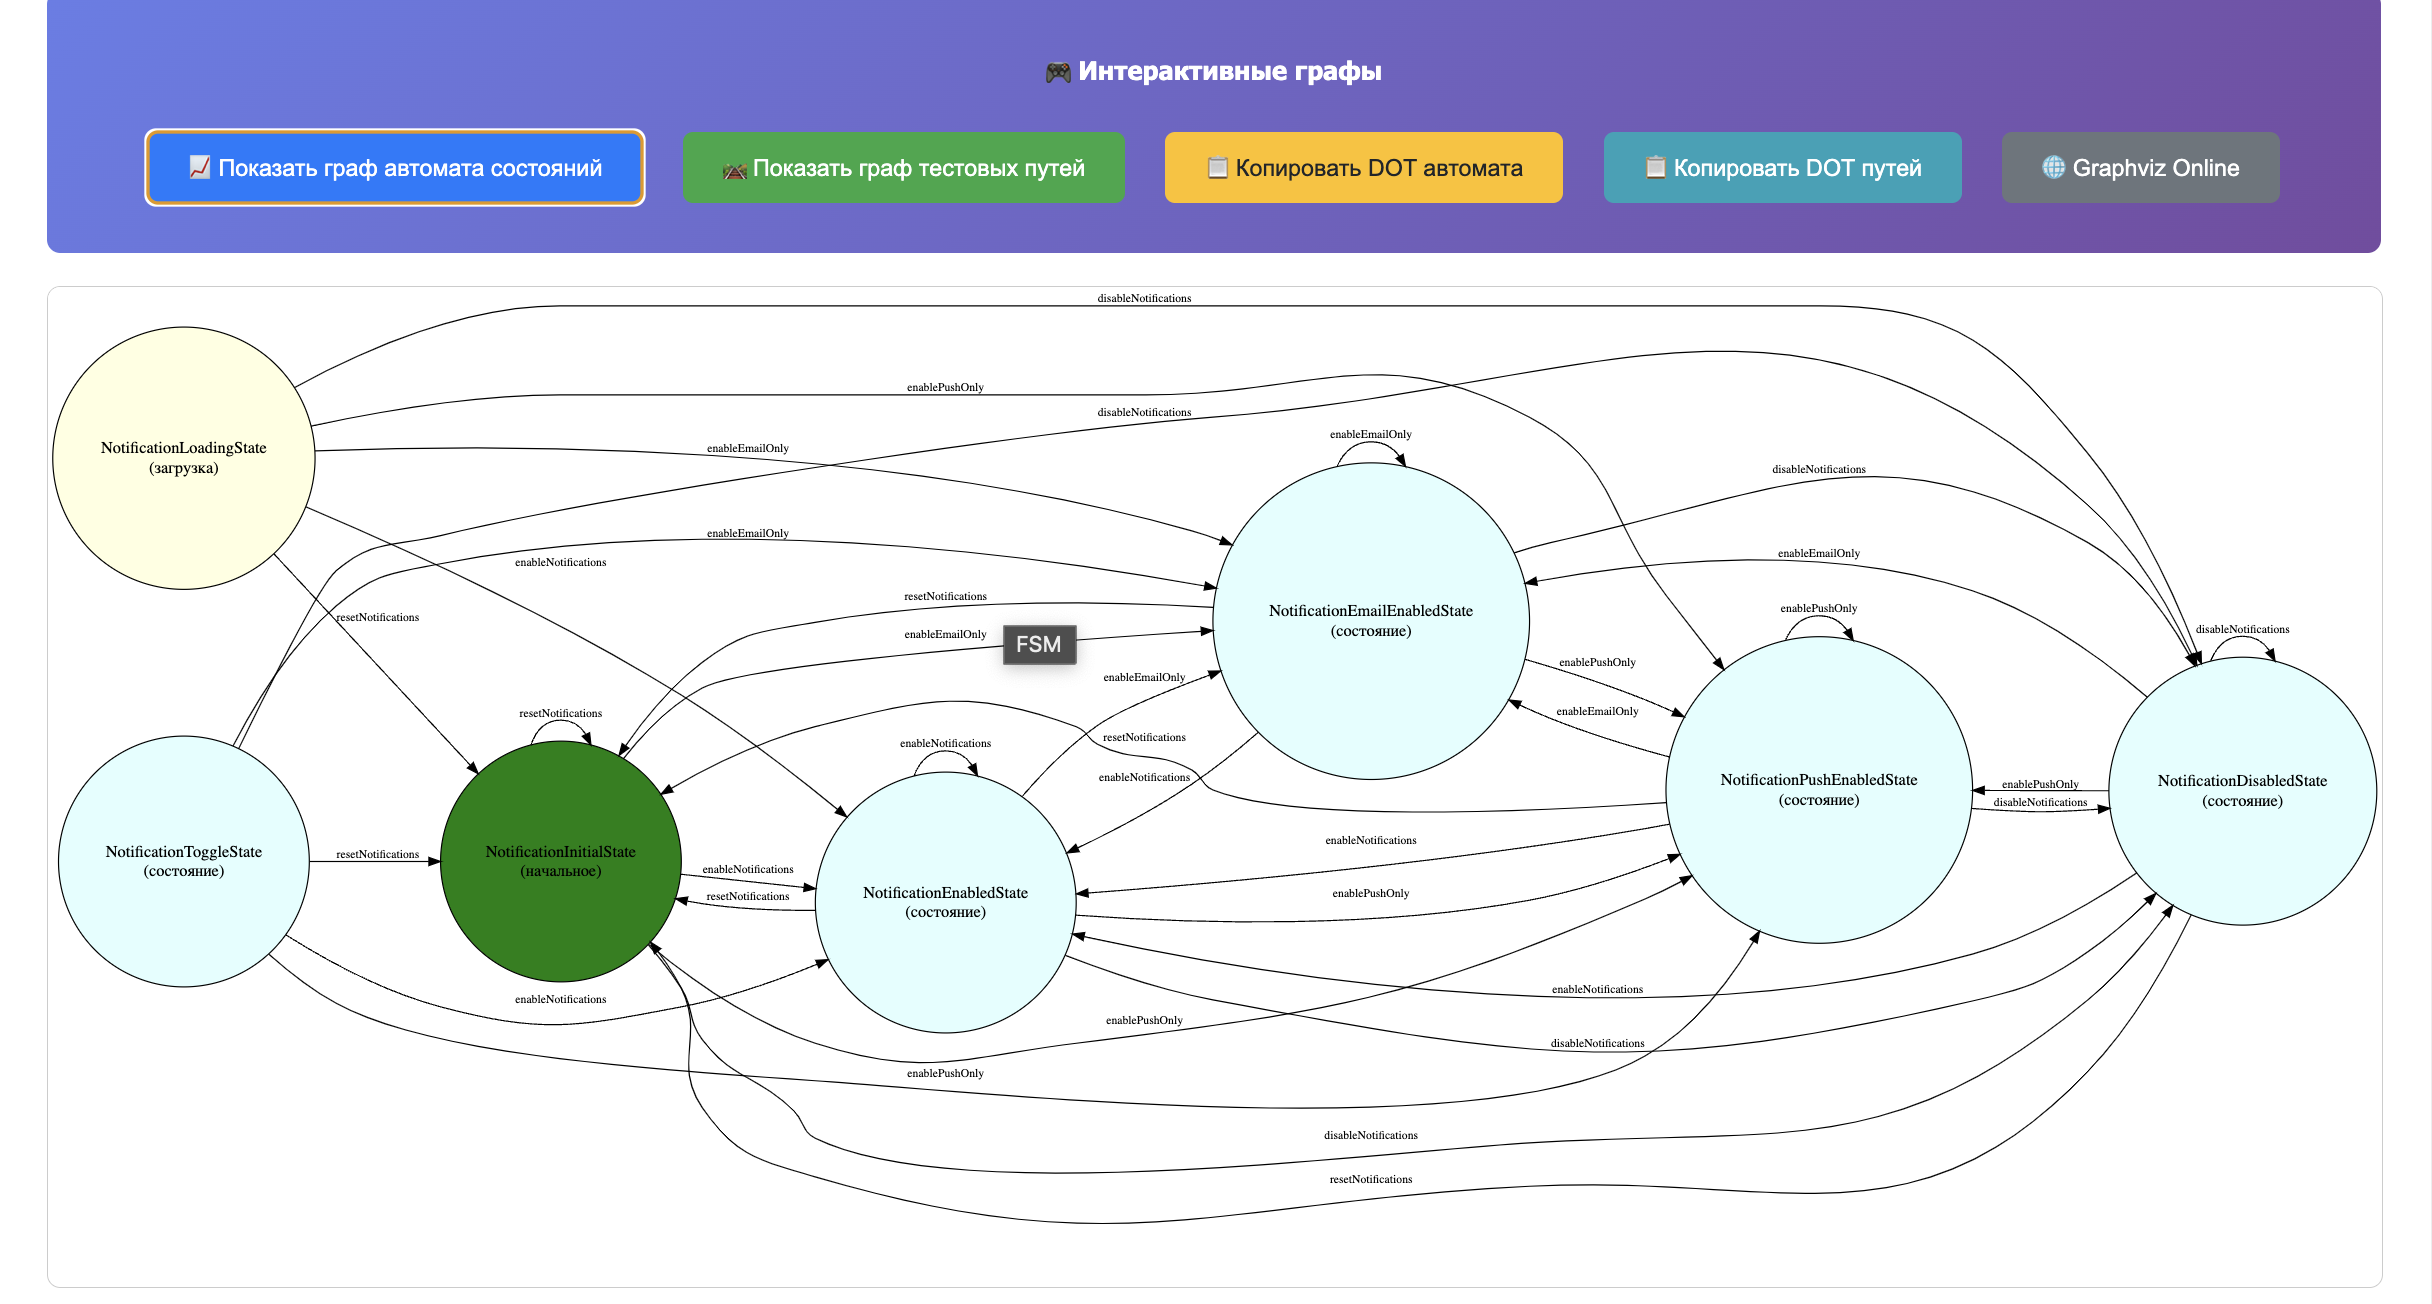
\includegraphics[width=0.7\textwidth]{images/cubit_4.png}
\caption{Атомат состояний кубита.}
\label{fig:cubit_more_info}
\end{figure}

\vspace{2cm}

\begin{figure}[!htb]
\centering
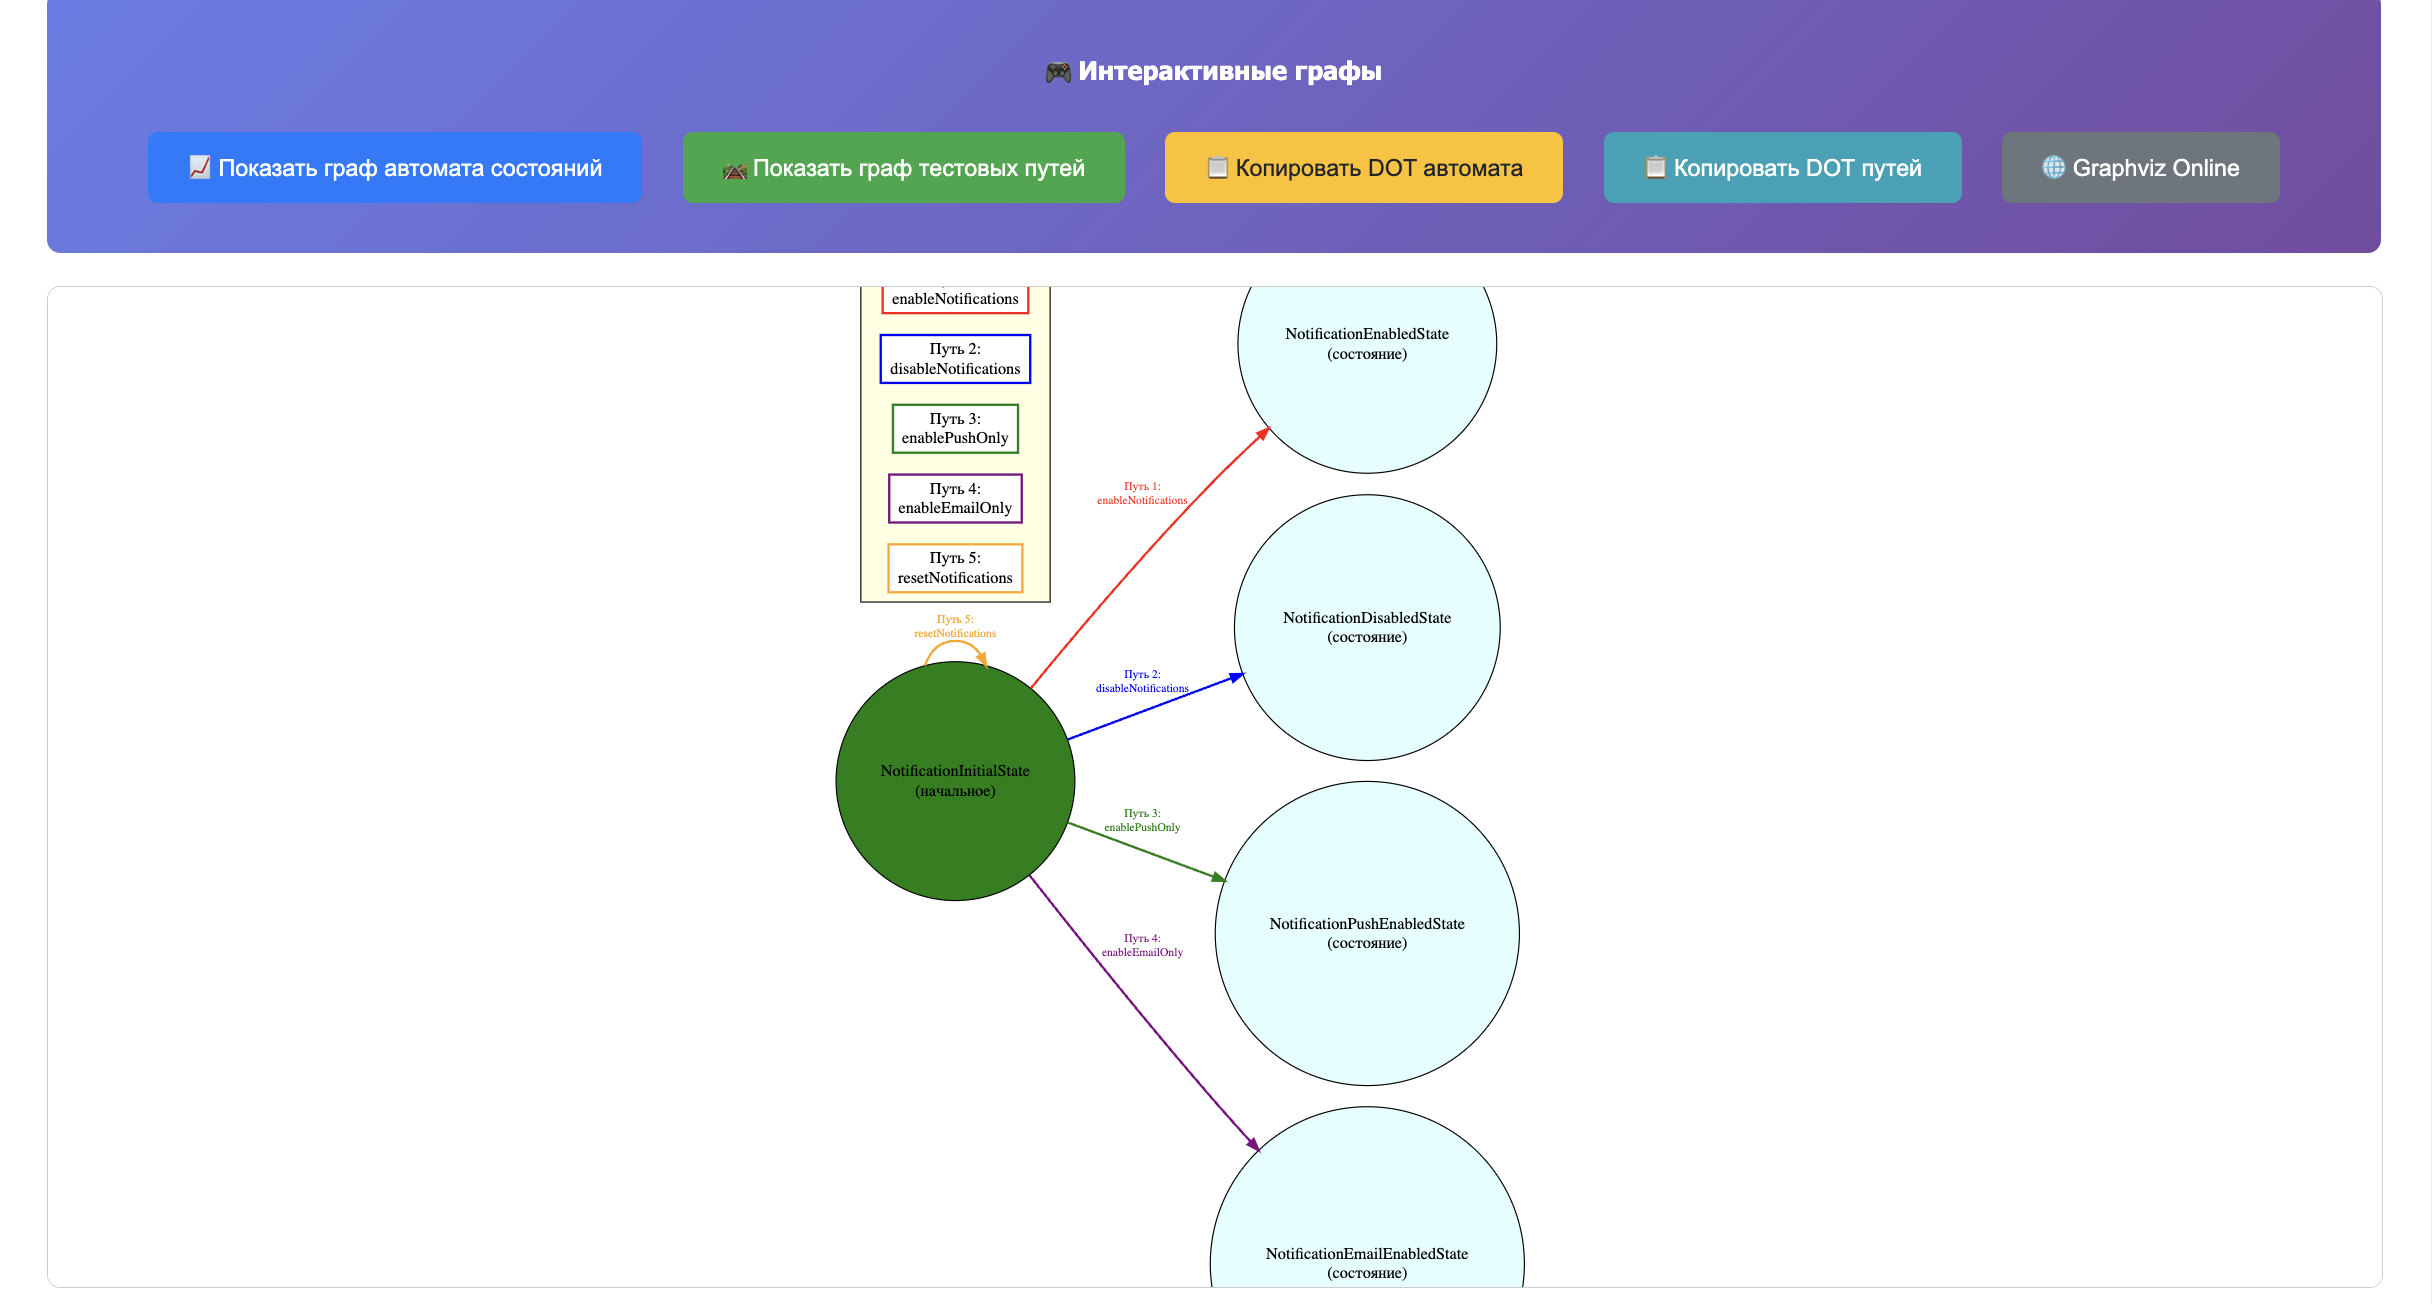
\includegraphics[width=0.7\textwidth]{images/cubit_5.png}
\caption{Тестовые множества кубита.}
\label{fig:cubit_more_info}
\end{figure}

% Конец отчета

\end{document}